\def\revtex{1}

\ifx\revtex\undefined

\documentclass[entropy,article,accept,oneauthor,pdftex]{Definitions/mdpi}

%\DeclareRobustCommand{\Eins}{\text{\usefont{U}{bbold}{m}{n}1}}
%\usepackage[dvipsnames]{xcolor}

%\usepackage{mathptmx}% http://ctan.org/pkg/mathptmx

%\usepackage{amssymb,amsthm,amsmath,bm}



\usepackage{mathbbol} %%%% for \mathds{1}


% For posting an early version of this manuscript as a preprint, you may use "preprints" as the journal and change "submit" to "accept". The document class line would be, e.g., \documentclass[preprints,article,accept,moreauthors,pdftex]{mdpi}. This is especially recommended for submission to arXiv, where line numbers should be removed before posting. For preprints.org, the editorial staff will make this change immediately prior to posting.

%--------------------
% Class Options:
%--------------------
%----------
% journal
%----------
% Choose between the following MDPI journals:
% acoustics, actuators, addictions, admsci, adolescents, aerospace, agriculture, agriengineering, agronomy, ai, algorithms, allergies, analytica, animals, antibiotics, antibodies, antioxidants, appliedchem, applmech, applmicrobiol, applnano, applsci, arts, asi, atmosphere, atoms, audiolres, automation, axioms, batteries, bdcc, behavsci, beverages, biochem, bioengineering, biologics, biology, biomechanics, biomedicines, biomedinformatics, biomimetics, biomolecules, biophysica, biosensors, biotech, birds, bloods, brainsci, buildings, businesses, cancers, carbon, cardiogenetics, catalysts, cells, ceramics, challenges, chemengineering, chemistry, chemosensors, chemproc, children, civileng, cleantechnol, climate, clinpract, clockssleep, cmd, coatings, colloids, compounds, computation, computers, condensedmatter, conservation, constrmater, cosmetics, crops, cryptography, crystals, curroncol, cyber, dairy, data, dentistry, dermato, dermatopathology, designs, diabetology, diagnostics, digital, disabilities, diseases, diversity, dna, drones, dynamics, earth, ebj, ecologies, econometrics, economies, education, ejihpe, electricity, electrochem, electronicmat, electronics, encyclopedia, endocrines, energies, eng, engproc, entropy, environments, environsciproc, epidemiologia, epigenomes, fermentation, fibers, fire, fishes, fluids, foods, forecasting, forensicsci, forests, fractalfract, fuels, futureinternet, futuretransp, futurepharmacol, futurephys, galaxies, games, gases, gastroent, gastrointestdisord, gels, genealogy, genes, geographies, geohazards, geomatics, geosciences, geotechnics, geriatrics, hazardousmatters, healthcare, hearts, hemato, heritage, highthroughput, histories, horticulturae, humanities, hydrogen, hydrology, hygiene, idr, ijerph, ijfs, ijgi, ijms, ijns, ijtm, ijtpp, immuno, informatics, information, infrastructures, inorganics, insects, instruments, inventions, iot, j, jcdd, jcm, jcp, jcs, jdb, jfb, jfmk, jimaging, jintelligence, jlpea, jmmp, jmp, jmse, jne, jnt, jof, joitmc, jor, journalmedia, jox, jpm, jrfm, jsan, jtaer, jzbg, kidney, land, languages, laws, life, liquids, literature, livers, logistics, lubricants, machines, macromol, magnetism, magnetochemistry, make, marinedrugs, materials, materproc, mathematics, mca, measurements, medicina, medicines, medsci, membranes, metabolites, metals, metrology, micro, microarrays, microbiolres, micromachines, microorganisms, minerals, mining, modelling, molbank, molecules, mps, mti, nanoenergyadv, nanomanufacturing, nanomaterials, ncrna, network, neuroglia, neurolint, neurosci, nitrogen, notspecified, nri, nursrep, nutrients, obesities, oceans, ohbm, onco, oncopathology, optics, oral, organics, osteology, oxygen, parasites, parasitologia, particles, pathogens, pathophysiology, pediatrrep, pharmaceuticals, pharmaceutics, pharmacy, philosophies, photochem, photonics, physchem, physics, physiolsci, plants, plasma, pollutants, polymers, polysaccharides, proceedings, processes, prosthesis, proteomes, psych, psychiatryint, publications, quantumrep, quaternary, qubs, radiation, reactions, recycling, regeneration, religions, remotesensing, reports, reprodmed, resources, risks, robotics, safety, sci, scipharm, sensors, separations, sexes, signals, sinusitis, smartcities, sna, societies, socsci, soilsystems, solids, sports, standards, stats, stresses, surfaces, surgeries, suschem, sustainability, symmetry, systems, taxonomy, technologies, telecom, textiles, thermo, tourismhosp, toxics, toxins, transplantology, traumas, tropicalmed, universe, urbansci, uro, vaccines, vehicles, vetsci, vibration, viruses, vision, water, wevj, women, world

%---------
% article
%---------
% The default type of manuscript is "article", but can be replaced by:
% abstract, addendum, article, book, bookreview, briefreport, casereport, comment, commentary, communication, conferenceproceedings, correction, conferencereport, entry, expressionofconcern, extendedabstract, datadescriptor, editorial, essay, erratum, hypothesis, interestingimage, obituary, opinion, projectreport, reply, retraction, review, perspective, protocol, shortnote, studyprotocol, systematicreview, supfile, technicalnote, viewpoint, guidelines, registeredreport, tutorial
% supfile = supplementary materials

%----------
% submit
%----------
% The class option "submit" will be changed to "accept" by the Editorial Office when the paper is accepted. This will only make changes to the frontpage (e.g., the logo of the journal will get visible), the headings, and the copyright information. Also, line numbering will be removed. Journal info and pagination for accepted papers will also be assigned by the Editorial Office.

%------------------
% moreauthors
%------------------
% If there is only one author the class option oneauthor should be used. Otherwise use the class option moreauthors.

%---------
% pdftex
%---------
% The option pdftex is for use with pdfLaTeX. If eps figures are used, remove the option pdftex and use LaTeX and dvi2pdf.

%=================================================================
% MDPI internal commands
%\ifx\revtex\undefined
%\maxdeadcycles=10000

%\maxdeadcycles=10000
\firstpage{1}
\makeatletter
\setcounter{page}{\@firstpage}
\makeatother
\pubvolume{1}
\issuenum{1}
\articlenumber{0}
\pubyear{2022}
\copyrightyear{2022}
\externaleditor{{Academic Editors: Gregg Jaeger and Jay Lawrence}
 }
\datereceived{30 December 2021}
\dateaccepted{11 March 2022}
\datepublished{}
\hreflink{https://doi.org/}
%------------------------------------------------------------------
% The following line should be uncommented if the LaTeX file is uploaded to arXiv.org
%\pdfoutput=1

%%%% If original paper need add "Retraction", please release the following command!!%%%%%%
%\retractiondate{Date Month Year} % For example, 13 October 2020
%\retractionnoticeyear{Year}
%\retractionnoticevolume{0}
%\retractionnoticeidnumber{0000}
%\retractionnoticedoi{10.3390/xxx}

%=================================================================
% Add packages and commands here. The following packages are loaded in our class file: fontenc, inputenc, calc, indentfirst, fancyhdr, graphicx, epstopdf, lastpage, ifthen, lineno, float, amsmath, setspace, enumitem, mathpazo, booktabs, titlesec, etoolbox, tabto, xcolor, soul, multirow, microtype, tikz, totcount, changepage, paracol, attrib, upgreek, cleveref, amsthm, hyphenat, natbib, hyperref, footmisc, url, geometry, newfloat, caption

%=================================================================
%% Please use the following mathematics environments: Theorem, Lemma, Corollary, Proposition, Characterization, Property, Problem, Example, ExamplesandDefinitions, Hypothesis, Remark, Definition, Notation, Assumption
%% For proofs, please use the proof environment (the amsthm package is loaded by the MDPI class).

%=================================================================
% Full title of the paper (Capitalized)
\Title{Generalized Householder Transformations}

% MDPI internal command: Title for citation in the left column
\TitleCitation{Generalized Householder Transformations}

% Author Orchid ID: enter ID or remove command
\newcommand{\orcidauthorA}{0000-0001-6554-2802} % Add \orcidA{} behind the author's name
%\newcommand{\orcidauthorB}{0000-0000-0000-000X} % Add \orcidB{} behind the author's name

% Authors, for the paper (add full first names)
\Author{Karl %MDPI: Please carefully check the accuracy of names and affiliations.
 Svozil \orcidA{}}

% MDPI internal command: Authors, for metadata in PDF
\AuthorNames{Karl Svozil}

% MDPI internal command: Authors, for citation in the left column
\AuthorCitation{Svozil, K.}
% If this is a Chicago style journal: Lastname, Firstname, Firstname Lastname, and Firstname Lastname.

% Affiliations / Addresses (Add [1] after \address if there is only one affiliation.)
\address[1]{%
Institute %MDPI: website link in affiliation should not be exist, please check and delete it.
 for Theoretical Physics, TU Wien, Wiedner Hauptstrasse 8-10/136, 1040 Vienna, Austria; svozil@tuwien.ac.at; \url{http://tph.tuwien.ac.at/~svozil}
}
% Contact information of the corresponding author
%\corres{Correspondence: svozil@tuwien.ac.at}

% Current address and/or shared authorship
%\firstnote{Current address: Affiliation 3}
%\secondnote{These authors contributed equally to this work.}
% The commands \thirdnote{} till \eighthnote{} are available for further notes

%\simplesumm{} % Simple summary

%\conference{} % An extended version of a conference paper

% Abstract (Do not insert blank lines, i.e. \\)
\abstract{The Householder transformation, allowing a rewrite of probabilities into expectations of dichotomic observables, is generalized in terms of its spectral decomposition. The dichotomy is modulated by allowing more than one negative eigenvalue or by abandoning binaries altogether, yielding generalized operator-valued arguments for contextuality. We also discuss a form of contextuality by the variation of the functional relations of the operators, in particular by additivity.}


% Keywords
\keyword{Householder transformation, expectation value, probability distribution, affine transformation}

% The fields PACS, MSC, and JEL may be left empty or commented out if not applicable
%\PACS{02.10.-v,05.45.Df,02.10.Ud,02.30.Cj}
%\MSC{}
%\JEL{}

%%%%%%%%%%%%%%%%%%%%%%%%%%%%%%%%%%%%%%%%%%
% Only for the journal Diversity
%\LSID{\url{http://}}

%%%%%%%%%%%%%%%%%%%%%%%%%%%%%%%%%%%%%%%%%%
% Only for the journal Applied Sciences:
%\featuredapplication{Authors are encouraged to provide a concise description of the specific application or a potential application of the work. This section is not mandatory.}
%%%%%%%%%%%%%%%%%%%%%%%%%%%%%%%%%%%%%%%%%%

%%%%%%%%%%%%%%%%%%%%%%%%%%%%%%%%%%%%%%%%%%
% Only for the journal Data:
%\dataset{DOI number or link to the deposited data set in cases where the data set is published or set to be published separately. If the data set is submitted and will be published as a supplement to this paper in the journal Data, this field will be filled by the editors of the journal. In this case, please make sure to submit the data set as a supplement when entering your manuscript into our manuscript editorial system.}

%\datasetlicense{license under which the data set is made available (CC0, CC-BY, CC-BY-SA, CC-BY-NC, etc.)}

%%%%%%%%%%%%%%%%%%%%%%%%%%%%%%%%%%%%%%%%%%
% Only for the journal Toxins
%\keycontribution{The breakthroughs or highlights of the manuscript. Authors can write one or two sentences to describe the most important part of the paper.}

%%%%%%%%%%%%%%%%%%%%%%%%%%%%%%%%%%%%%%%%%%
% Only for the journal Encyclopedia
%\encyclopediadef{Instead of the abstract}
%\entrylink{The Link to this entry published on the encyclopedia platform.}
%%%%%%%%%%%%%%%%%%%%%%%%%%%%%%%%%%%%%%%%%%

%\usepackage{amsmath,amssymb}
%\usepackage{mathbbol} %%%% for \mathds{1}
%\DeclareFontFamily{U}{bbold}{}
%\DeclareFontShape{U}{bbold}{m}{n}
% {
% <-5.5> s*[1.069] bbold5
% <5.5-6.5> s*[1.069] bbold6
% <6.5-7.5> s*[1.069] bbold7
% <7.5-8.5> s*[1.069] bbold8
% <8.5-9.5> s*[1.069] bbold9
% <9.5-11> s*[1.069] bbold10
% <11-15> s*[1.069] bbold12
% <15-> s*[1.069] bbold17
% }{}


 \begin{document}
%%%%%%%%%%%%%%%%%%%%%%%%%%%%%%%%%%%%%%%%%%
%\setcounter{section}{-1} %% Remove this when starting to work on the template.



\else

\documentclass[%
 %    reprint,
   twocolumn,
 %superscriptaddress,
 %groupedaddress,
 %unsortedaddress,
 %runinaddress,
 %frontmatterverbose,
 % preprint,
 % showpacs,
 % showkeys,
 % preprintnumbers,
 % nofootinbib,
 %nobibnotes,
 %bibnotes,
 amsmath,amssymb,
 aps,
 % prl,
 pra,
 % prb,
 % rmp,
 %prstab,
 %prstper,
  longbibliography,
 %floatfix,
 %lengthcheck,%
 ]{revtex4-2}

%\usepackage{cdmtcs-pdf}




\usepackage[dvipsnames]{xcolor}

\usepackage{mathptmx}% http://ctan.org/pkg/mathptmx

\usepackage{amssymb,amsthm,amsmath,bm}

\usepackage{tikz}
\usetikzlibrary{calc,decorations.pathreplacing,decorations.markings,positioning,shapes,snakes}
%\usetikzlibrary{calc,decorations.pathreplacing,decorations.markings,positioning,shapes,snakes,external}
%\tikzexternalize

\usepackage[breaklinks=true,colorlinks=true,anchorcolor=blue,citecolor=blue,filecolor=blue,menucolor=blue,pagecolor=blue,urlcolor=blue,linkcolor=blue]{hyperref}
\usepackage{graphicx}% Include figure files
\usepackage{url}

%%%%%%%%%%%%%%%%%%%%%%%%%%%%%
%\usepackage{iftex}
\ifxetex
%
% XeLaTeX
%
\usepackage{fontspec}
\usepackage{fontspec}
\setmainfont{Garamond}
\setsansfont{Garamond}
%
\fi
%%%%%%%%%%%%%%%%%%%%%%%%%%%%%

\usepackage{mathbbol} %%%% for \mathds{1}

\begin{document}

\title{Generalized Householder transformations}


\author{Karl Svozil}
\email{svozil@tuwien.ac.at}
\homepage{http://tph.tuwien.ac.at/~svozil}

\affiliation{Institute for Theoretical Physics,
TU Wien,
Wiedner Hauptstrasse 8-10/136,
1040 Vienna,  Austria}


\date{\today}

\begin{abstract}
The Householder transformation, allowing a rewrite of probabilities into expectations of dichotomic observables, is generalized in terms of its spectral decomposition. The dichotomy is modulated by allowing more than one negative eigenvalue or by abandoning binaries altogether, yielding generalized operator-valued arguments for contextuality. We also discuss a form of contextuality by the variation of the functional relations of the operators, in particular by additivity.
\end{abstract}

\keywords{Householder transformation}
%\pacs{02.10.-v,05.45.Df,02.10.Ud,02.30.Cj}

\maketitle

\fi

\section{From probabilities to expectations}

A standard way to recast classical probabilities $p \in \left[ 0,1 \right]$ into expectations $E \in \left[ -a,a \right]$
of two-valued---indeed, $\left\{ -a,a \right\}$--valued, observables---is in terms of affine transformations $E_a (p) = a(2p - 1)$,
amounting to a doubling of the probability and a shift by minus one, times $a$.
(Often the physical units in terms of which observables are measured are chosen to be such that $a=1$.)
This can be motivated by the linearity of classical probabilities which can be
defined as the convex polytope of ``extreme cases'' or truth assignments, symbolized by two-valued measures $v \in \left\{ 0,1 \right\}$.

It is an interesting property of quantum mechanics that the dimensionality $n\in \mathbb{N}$
of the associated Hilbert space $\mathbb{C}^n$ is determined by the finest resolution of its contexts or
``maximal observables'': a context contains an exhaustive (aka maximal or complete) set of mutually
exclusive elementary observables.
Each one of these elementary observables is identifiable by an elementary proposition, which in
turn is formalizable by a one dimensional orthogonal projection operator $\textsf{\textbf{F}}$ that is both self-adjoint as well as idempotent;
that is, $\textsf{\textbf{F}}=\textsf{\textbf{F}}^\dagger$,
where $\dagger$ represents the Hermitian adjoint (aka conjugate), and $\textsf{\textbf{F}}^2 = \textsf{\textbf{F}}$,
respectively.
Thereby, $n=2$ associated with dichotomic observables just represents a bound from below for nontrivial predictions.
But for $n>2$ there are no preferred Leibnizian ``dyadic'' schemes, such as bases, to represent and encode
vectors or pure states in $n$-dimensional Hilbert spaces:
neither the dimensionality---suggesting rather an $n$--ary encoding---nor the scalar product (nor completeness) yields any such preference;
albeit arbitrary rotations (unitary transformations) in $n$ dimensions can be obtained (and parameterized~\cite{murnaghan})
by the serial composition of rotations (unitary transformations) in two-dimensional subspaces of $\mathbb{C}^n$.

Therefore, it might not be too far-fetched to ask which constructions might provide generalizations
of the aforementioned affine transformations in arbitrary dimensions.
In particular, what presents, at least to some degree of semblance, the quantum mechanical counterparts of classical expectations from probabilities mentioned earlier?

An answer can be given in terms of
the so-called Householder transformations (e.g., Ref.~\cite{Horn-Johnson-MatrixAnalysis}) as follows.
The respective techniques are well developed but may be less known in the quantum foundations community,
so a review at the beginning seems in order.
We shall then proceed to modifications of Householder transformations to nondichotomic, multiple eigenvalues.

Let $\vert {\bf x} \rangle \in \mathbb{C}^n$ be a nonzero vector and
$\textsf{\textbf{F}}_{\bf x} =  ( \langle {\bf x} \vert   {\bf x} \rangle )^{-1} \vert {\bf x} \rangle \langle  {\bf x}  \vert$
the respective orthogonal projection operator.
The Householder transformation $\textsf{\textbf{U}}_{\bf x}$ is defined by
\begin{equation}
\textsf{\textbf{U}}_{\bf x}
=
\Eins - 2 \textsf{\textbf{F}}_{\bf x} =
\Eins - 2 ( \langle {\bf x} \vert   {\bf x} \rangle )^{-1} \vert {\bf x} \rangle \langle  {\bf x}  \vert
.
\end{equation}
 If  $\vert {\bf x} \rangle $ is a unit vector, then
$\textsf{\textbf{U}}_{\bf x}
=
\Eins - 2  \vert {\bf x} \rangle \langle  {\bf x}  \vert$.

The following properties can be asserted by direct proofs:
\begin{itemize}
\item[(i)]
$\textsf{\textbf{U}}_{\bf x}$ is Hermitian; that is,
$
\textsf{\textbf{U}}_{\bf x} = \textsf{\textbf{U}}_{\bf x}^\dagger
$;

\item[(ii)]
$\textsf{\textbf{U}}_{\bf x}$ is unitary; that is,
\begin{equation}
\begin{split}
\textsf{\textbf{U}}_{\bf x}  \textsf{\textbf{U}}_{\bf x}^\dagger
=
\textsf{\textbf{U}}_{\bf x}^\dagger  \textsf{\textbf{U}}_{\bf x}
=
\textsf{\textbf{U}}_{\bf x}  \textsf{\textbf{U}}_{\bf x}
\\
=
\left(\Eins - 2 ( \langle {\bf x} \vert   {\bf x} \rangle )^{-1} \vert {\bf x} \rangle \langle  {\bf x}  \vert\right)
\left(\Eins - 2 ( \langle {\bf x} \vert   {\bf x} \rangle )^{-1} \vert {\bf x} \rangle \langle  {\bf x}  \vert\right)
\\
= \Eins  - 4 ( \langle {\bf x} \vert   {\bf x} \rangle )^{-1} \vert {\bf x} \rangle \langle  {\bf x}  \vert
+ 4 ( \langle {\bf x} \vert   {\bf x} \rangle )^{-1} \vert {\bf x} \rangle \langle  {\bf x}  \vert =
\Eins
.
\end{split}
\end{equation}

\item[(iii)]
Hence $\textsf{\textbf{U}}_{\bf x}$ is involutory:
$\textsf{\textbf{U}}_{\bf x}^{-1} =  \textsf{\textbf{U}}_{\bf x}$.
\index{involution}

\item[(iv)]
The eigensystem of $\textsf{\textbf{U}}_{\bf x}$ has two eigenvalues $\pm 1$:
\begin{itemize}
\item[$-1$:]
$\,$For the eigenvector $ \vert {\bf x} \rangle$ of    $\textsf{\textbf{U}}_{\bf x}$,
with
$\textsf{\textbf{U}}_{\bf x}\vert {\bf x} \rangle
=
\left(\Eins - 2 ( \langle {\bf x} \vert   {\bf x} \rangle )^{-1} \vert {\bf x} \rangle \langle  {\bf x}  \vert\right)\vert {\bf x} \rangle
= \vert {\bf x} \rangle- 2 \vert {\bf x} \rangle =- \vert {\bf x} \rangle$
the associated eigenvalue is $-1$.
\item[$+1$:]
$\,$The remaining $n-1$ mutually orthogonal eigenvectors span the $n-1$ dimensional subspace orthogonal to $\vert {\bf x} \rangle $.
Every vector in that subspace has eigenvalue $+1$.
(For $n>2$ the spectrum is degenerate.)
\end{itemize}

Stated differently: for all vectors orthogonal to $\vert {\bf x} \rangle $ the
Householder transformation $\textsf{\textbf{U}}_{\bf x}$ acts as identity;
and for $\vert {\bf x} \rangle $ the
Householder transformation $\textsf{\textbf{U}}_{\bf x}$
acts as a reflection on the one-dimensional subspace spanned by $\vert {\bf x} \rangle $.

\item[(v)]
Since the determinant of a matrix is the product of its eigenvalues,
the determinant of a Householder transformation is $-1$.

\item[(vi)]
If
$\mathcal{C}= \{\vert {\bf e}_1\rangle ,
\vert  {\bf e}_2\rangle , \ldots , \vert {\bf e}_n\rangle \}$
is an orthonormal basis formalizing a context, then the succession
of the respective Householder transformations renders negative unity; that is,
\begin{equation}
\begin{split}
\textsf{\textbf{U}}_{{\bf e}_1} \textsf{\textbf{U}}_{{\bf e}_2} \cdots \textsf{\textbf{U}}_{{\bf e}_n}
=
\left(\Eins - 2  \vert {\bf e}_1 \rangle \langle  {\bf e}_1  \vert\right)
\left(\Eins - 2  \vert {\bf e}_2 \rangle \langle  {\bf e}_2  \vert\right)
\cdots
\left(\Eins - 2  \vert {\bf e}_n \rangle \langle  {\bf e}_n  \vert\right) \\
=
\Eins - 2 \underbrace{\left( \vert {\bf e}_1 \rangle \langle  {\bf e}_1 \vert +
 \vert {\bf e}_2 \rangle \langle  {\bf e}_2  \vert +
\cdots
+  \vert {\bf e}_n \rangle \langle  {\bf e}_n  \vert\right)}_{\Eins }=
-\Eins .
\end{split}
\label{2021-hh-minusunity}
\end{equation}
\end{itemize}




For the sake of an example, let
 $\vert {\bf z} \rangle =\begin{pmatrix}1,1\end{pmatrix}^\intercal$,
so that the corresponding Householder transformation can be written in matrix form as
\[
\textsf{\textbf{U}}_{\bf z}
= \Eins - 2  ( \langle {\bf z} \vert   {\bf z} \rangle )^{-1} \vert {\bf z} \rangle \langle  {\bf z}  \vert
\equiv \begin{pmatrix}1&0\\0&1\end{pmatrix} -2(2)^{-1} \begin{pmatrix}1&1\\1&1\end{pmatrix}
= -\begin{pmatrix}0&1\\1&0\end{pmatrix}.\]


Take
 $\vert {\bf x} \rangle =\begin{pmatrix}2,1\end{pmatrix}^\intercal$,
so that
 $\vert {\bf y} \rangle =-\begin{pmatrix}1,2\end{pmatrix}^\intercal$:
this ``reflected'' vector $\vert {\bf y} \rangle$ and the original vector $\vert {\bf x} \rangle$
have the same length or norm.
The component of $\vert {\bf y} \rangle$  along $\vert {\bf z} \rangle$ is reversed, whereas its component orthogonal to
$\vert {\bf z} \rangle$ remains the same.
This situation is depicted in Figure~\ref{2021-mm-fdvs-householder}.



Because of (iii), if $\vert {\bf x} \rangle \neq \vert {\bf y} \rangle$ are two vectors  in $\mathbb{R}^n$
with identical length or norm
$\| {\bf x} \| = \| {\bf y} \|$
then there exists a remarkable ``symmetry delivered by'' a Householder transformation $\textsf{\textbf{U}}_{\bf z}$ such that
$\textsf{\textbf{U}}_{\bf z} \vert {\bf x} \rangle =  \vert {\bf y} \rangle$
and
$\textsf{\textbf{U}}_{\bf z}\textsf{\textbf{U}}_{\bf z} \vert {\bf x} \rangle =  \textsf{\textbf{U}}_{\bf z}\vert {\bf y} \rangle
=  \vert {\bf x} \rangle$.
For this to hold the vector $\vert {\bf z} \rangle$ needs to be a  vector equal to $\vert {\bf x} \rangle - \vert {\bf y} \rangle$:
$  \left( \Eins - 2  ( \langle {\bf z} \vert   {\bf z} \rangle )^{-1} \vert {\bf z} \rangle \langle  {\bf z}  \vert  \right) \vert {\bf x} \rangle =  \vert {\bf y} \rangle
$
and
$ \vert {\bf x} \rangle  =   \left( \Eins - 2  ( \langle {\bf z} \vert   {\bf z} \rangle )^{-1}\vert {\bf z} \rangle \langle  {\bf z}  \vert  \right) \vert {\bf y} \rangle
$,
resulting in
$( \langle {\bf z} \vert   {\bf z} \rangle )^{-1} \vert {\bf z} \rangle \langle  {\bf z}  \vert  \left( \vert {\bf x} \rangle  - \vert {\bf y} \rangle \right)
= \vert {\bf x} \rangle  - \vert {\bf y} \rangle
$, and thus $\vert {\bf z} \rangle =  \vert {\bf x} \rangle  - \vert {\bf y} \rangle$.
(For $\vert {\bf x} \rangle = \vert {\bf y} \rangle$ identify with $\vert {\bf z} \rangle$ a vector orthogonal to $\vert {\bf x} \rangle = \vert {\bf y} \rangle$.)
This is not true for $\mathbb{C}^n$, as for instance, there exists no $ \vert {\bf z} \rangle $ which would render
$\textsf{\textbf{U}}_{\bf z} \vert {\bf x} \rangle =  i \vert {\bf x} \rangle$ for nonzero  $ \vert {\bf x} \rangle $,
and an additional unitary transformation is required.

This gives rise to the orthonormalizion of a set of $k$ linear independent nonzero vectors
$\mathcal{S}=\{\vert {\bf s}_1\rangle ,
\vert  {\bf s}_2\rangle , \ldots , \vert {\bf s}_k\rangle \}$   in $\mathbb{R}^n$
by taking some orthonormal basis
$\mathcal{C}=\{{\bf e}_1,  {\bf e}_2, \ldots , {\bf e}_n\}\equiv \{\vert {\bf e}_1\rangle ,
\vert  {\bf e}_2\rangle , \ldots , \vert {\bf e}_n\rangle \}$,
choosing $k$ vectors thereof---say, the first $k$ vectors of the standard Cartesian coordinate system---and identifying
$\vert {\bf s}_i\rangle$ with $\vert {\bf x}_i\rangle$,
and (the extra factor $\| {\bf s}_i \|$ serves to make the vector of equal length or norm)
$\vert {\bf y}_i\rangle$ with $\| {\bf s}_i \| \vert {\bf e}_i\rangle$,
thereby constructing a Householder transformation followed by normalization (through division by $\| {\bf s}_i \|$)
$\textsf{\textbf{U}}_{{\bf z}_i}$ of $\vert {\bf s}_i\rangle \stackrel{\textsf{\textbf{U}}_{{\bf z}_i}}{\mapsto} \vert {\bf e}_i\rangle$
with respective
$\vert {\bf z}_i\rangle = \vert {\bf s}_i\rangle  - \| {\bf s}_i \| \vert {\bf e}_i\rangle$.
This kind of orthonormalization may yield a span ``outside'' of the  subspace  spanned by the ``original'' vectors.


\begin{figure}
\begin{center}%
\resizebox{0.4\textwidth}{!}{
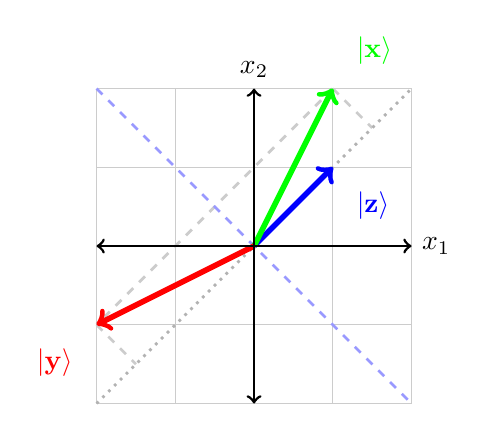
\begin{tikzpicture}  [scale=1]

\tikzstyle{every path}=[line width=1pt]

\newdimen\ms
\ms=0.1cm
\tikzstyle{s1}=[color=red,rectangle,inner sep=3.5]
\tikzstyle{c3}=[circle,inner sep={\ms/8},minimum size=4*\ms]
\tikzstyle{c2}=[circle,inner sep={\ms/8},minimum size=3*\ms]
\tikzstyle{c1}=[circle,inner sep={\ms/8},minimum size=2*\ms]
\tikzstyle{cs1}=[circle,inner sep={\ms/8},minimum size=1*\ms]



% Define positions of all observables


\coordinate (zero) at (0,0);
\coordinate (v) at (1,1);
\coordinate (x) at (1,2);
\coordinate (y) at (-2,-1);

% draw grid

 \draw[dashed, line width=1pt,gray!40](x)--(y);
 \draw[dashed, line width=1pt,gray!40](x)--(1.5,1.5);
 \draw[dashed, line width=1pt,gray!40](y)--(-1.5,-1.5);
 \draw[thin,gray!40] (-2,-2) grid (2,2);


% draw vectors

 \draw[dashed, line width=1pt,blue!40](-2,2)--(2,-2);
 \draw[dotted, line width=1pt,gray!60](-2,-2)--(2,2);




 \draw[->,line width=2pt,blue](zero)--(v) node[label=below right:{$\vert {\bf z}\rangle $}] {};

 \draw[->,line width=2pt,green](zero)--(x) node[label=above right:{$\vert {\bf x}\rangle $}] {};

 \draw[->,line width=2pt,red](zero)--(y) node[label=below left:{$\vert {\bf y}\rangle $}] {};

% draw a coordinate system


  \draw[<->] (-2,0)--(2,0) node[right]{$x_1$};
  \draw[<->] (0,-2)--(0,2) node[above]{$x_2$};

\end{tikzpicture}
}
\end{center}
\caption{\label{2021-mm-fdvs-householder}
Depiction of the Householder transformation $\textsf{\textbf{U}}_{\bf z}$
with
$\vert {\bf z} \rangle =\begin{pmatrix}1,1\end{pmatrix}^\intercal$
acting on a vector $\vert {\bf x} \rangle =\begin{pmatrix}2,1\end{pmatrix}^\intercal$.
The resulting ``reflected'' vector $\vert {\bf y} \rangle = \textsf{\textbf{U}}_{\bf z} \vert {\bf x} \rangle$
and the original vector $\vert {\bf x} \rangle$
have the same length or norm.
Its component along $\vert {\bf z} \rangle$ is reversed, whereas its component orthogonal to
$\vert {\bf z} \rangle$ remains the same.}
\end{figure}

Cabello has used the Householder transformation to argue for what he calls
``state-independent quantum contextuality''~\cite{cabello:210401,PhysRevLett.103.050401}.
Thereby, in a first construction step, all $2^{16}$ possible classical value assignments
of the elementary propositions $a_1, \cdots ,a_{16} \in \left\{ -1,1\right\}$
depicted in Figure~\ref{2018-m-ch-fdlvs-ksc}, grouped into the nine contexts
$\mathcal{C}_1, \ldots , \mathcal{C}_9$ are enumerated.
In a second step, for each one of the nine contexts, the respective four (per context) possible classical value assignments
of the elementary propositions are multiplied.
In a third step these nine (per  classical value assignment) products are added together.
As a result each of the $2^{16}$ valuations yields a number, an integer between the algebraically maximal values $-9$ and $9$---bounds obtained from the number of the (nine) contexts involved.

As it turns out 9216 value assignments are rendering the number $-7$, and none rendering $-8$ or $-9$.
But these classical value assignments are not admissible~\cite{2015-AnalyticKS} in the sense of~(iv) mentioned earlier---an {\em ad hoc} assumption---as
there does not exist a classical (non-contextual) two-valued $\{0,1\}$-state on these 18 observables in 9 contexts
which would allow a translation into a $\{-1,1\}$-value assignment such that each context contains exactly one
element that is assigned the value ``$-1$'' and all other elements of that context are assigned the value ``$+1$''.
For the sake of anecdotal demonstration (no proof), Figure~\ref{2018-m-ch-fdlvs-ksc} contains an ``illegal'' value assignment that renders the maximal value 7
of the sum of the products of all value assignments within the nine contexts.

Indeed, relative to admissibility, state-independent quantum contextuality
is a corollary of the Kochen-Specker theorem for configurations without any two-valued states.
Because in this case no (homomorphic) translation from admissible two-valued $\{0,1\}$-states $p$
into two-valued $\{-1,1\}$-observables $E$ with affine $E(p) = 2p - 1$ exist.

In the relaxed case admissibility can be violated---in particular, by an {\em ad hoc}  breach of exclusivity, thereby
allowing more than one value assignment ``$1$'' per context---while at the same time maintaining noncontextuality
(at the intertwining observables).
State-independent quantum contextuality can only be counterfactually postulated
if and only if the quantum Householder transformation-based
predictions---equal to the (modulus of) the number of contexts involved---are {\it not} realizable by classical noncontextual,
admissible or inadmissible value assignments.
Therefore,
the sum of all products of observables within all contexts should not
reach its algebraic maximal obtainable value.
(As noted earlier this maximal obtainable value is just the number of contexts involved.)
That implies that it should not
be possible to require the number of noncontextual value assignments ``$-1$'' within each given context to be odd.
As a result, strictly bi-connected (indeed even-number connected)
Kochen-Specker configurations involving an odd number of contexts always
exhibit state-independent quantum contextuality.
The proof is similar to the indirect parity proof of the Kochen-Specker theorem for the configuration
introduced by Cabello, Estebaranz-Garc{\'{i}}a-Alcaine~\cite{cabello-96}:
for a proof by contradiction, suppose the products of observables within all contexts are multiplied.
On the one hand, since by assumption, there are odd contexts, each contributing a factor $-1$, this
number---the odd product of products---should be $-1$.
But on the other hand, by bi- or even-connectivity, the product of products contains only squares
or even multiples of factors, which return $+1$---a complete contradiction.


Figure~\ref{2018-m-ch-fdlvs-ksc} contains an instance of classical inadmissible value assignment that cannot reach the
algebraic maximal sum, as would be required by the quantum Householder transformation prediction.
Further methods to obtain such configurations based on parity proofs are discussed by Waegell, Aravind, Megill,
and Pavi{\v{c}}i{\'{c}}~\cite{Pavicic-2011a,Pavicic-2017,Pavii2018}.
The Greenberger-Horne-Zeilinger operator theorem is based on a similar argument~\cite{ghz,svozil-2020-ghz}.


For all other multi-context configurations allowing
two-valued states---even with a nonseparable or unital set of two-valued states---the translation from
$\{0,1\}$-states into two-valued $\{-1,1\}$-observables
there is no state-independent quantum contextuality.
For other operator-valued assignments see, for instance, references~\cite{PhysRevLett.103.050401,Yu2015}.



I shall leave open the question of how convincing and applicable to counterfactual arguments such inadmissible value
assignments---even in their operator-valued translations---might be.
At the moment, I am inclined to understand such situations and configurations rather in terms of
the Kochen-Specker theorem~\cite{kochen1}, or quantitatively about the associated
chromatic number; that is, in terms of how many colors are needed
to separate elements in the respective contexts~\cite{Shekarriz-Svozil}.

A quantum realization of the Cabello, Estebaranz-Garc{\'{i}}a-Alcaine~\cite{cabello-96,cabello:210401}
configuration is a faithful orthogonal representation~\cite{lovasz-79,lovasz-89,Portillo-2015}
that includes 18 unit vectors or associated one-dimensional orthogonal projection operators
$\textsf{\textbf{F}}_i  = \vert a_i \rangle \langle a_i \vert$, with $1 \le i \le 18$
as vector labels of the hypergraph depicted in Figure~\ref{2018-m-ch-fdlvs-ksc}; whereby adjacency of
hypergraph vertices is translated into orthogonality of the vectors serving as their labels.

As we have learned in~(vi), Equation~(\ref{2021-hh-minusunity}),
within each one of the nine contexts the products of these elementary observables is $-1$.
Adding together all nine products of the nine contexts yields the algebraically maximal sum $-1$ for all quantum value assignments.
This is in contradiction to the classical predictions which never yield $-8$ or $-9$.
Note that this argument requires the counterfactual existence of all quantum observables
$\textsf{\textbf{F}}_i  = \vert a_i \rangle \langle a_i \vert$, even as only a single one context (from nine contexts
$\mathcal{C}_1, \ldots , \mathcal{C}_9$) is operationally accessible.


\begin{figure}
\begin{center}
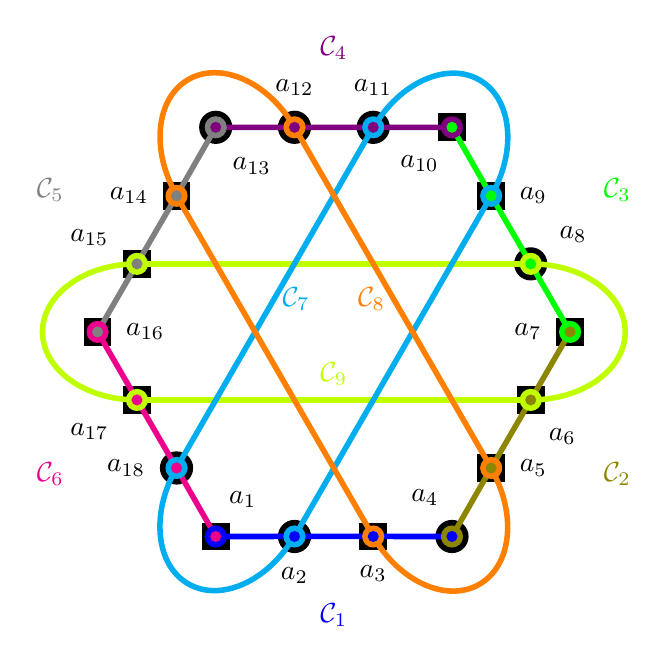
\begin{tikzpicture}  [scale=0.6]

        \tikzstyle{every path}=[line width=2pt]
        \tikzstyle{s3}=[rectangle,inner sep=1pt,minimum size=10pt]
        \tikzstyle{c3}=[circle,inner sep=2pt,minimum size=12pt]
        \tikzstyle{c2}=[circle,inner sep=2pt,minimum size=8pt]
        \tikzstyle{c1}=[circle,inner sep=1pt,minimum size=4pt]
        %\tikzstyle{s1}=[rectangle,minimum size=9]
        \tikzstyle{l1}=[draw=none,circle,minimum size=35]
        \tikzstyle{l2}=[draw=none,circle,minimum size=12]

        % Define positions of all observables
        \path
              (240:5) coordinate(1)
              (-0.833,-4.33) coordinate(2)
              (0.833,-4.33) coordinate(3)
              (300:5) coordinate(4)
              (3.33,-2.88) coordinate(5)
              (4.167,-1.44) coordinate(6)
              (0:5) coordinate(7)
              (4.167,1.44) coordinate(8)
              (3.33,2.88) coordinate(9)
              (60:5) coordinate(10)
              (0.833,4.33) coordinate(11)
              (-0.833,4.33) coordinate(12)
              (120:5) coordinate(13)
              (-3.33,2.88) coordinate(14)
              (-4.167,1.44) coordinate(15)
              (180:5) coordinate(16)
              (-4.167,-1.44) coordinate(17)
              (-3.33,-2.88) coordinate(18);

\node[draw=none,color=blue] at (0,-6)      {$\mathcal{C}_1$};
\node[draw=none,color=olive] at (6,-3)       {$\mathcal{C}_2$};
\node[draw=none,color=green] at (6,3)      {$\mathcal{C}_3$};
\node[draw=none,color=violet] at (0,6)     {$\mathcal{C}_4$};
\node[draw=none,color=gray] at (-6,3)      {$\mathcal{C}_5$};
\node[draw=none,color=magenta] at (-6,-3)  {$\mathcal{C}_6$};
\node[draw=none,color=cyan] at (-0.8,0.7)  {$\mathcal{C}_7$};
\node[draw=none,color=orange] at (0.8,0.7) {$\mathcal{C}_8$};
\node[draw=none,color=lime] at (0,-0.9)    {$\mathcal{C}_9$};



        \draw (1) coordinate[s3,fill=red!70,color=black,label=85:$a_1$];
        \draw (2) coordinate[c3,fill=green!70,color=black,label=270:$a_2$];
        \draw (3) coordinate[s3,fill=red!70,color=black,label=270:$a_3$];
        \draw (4) coordinate[c3,fill=green!70,color=black,label=95:$a_4$];
        \draw (5) coordinate[s3,fill=red!70,color=black,label=0:$a_5$];
        \draw (6) coordinate[s3,fill=red!70,color=black,label=290:$a_6$];
        \draw (7) coordinate[s3,fill=red!70,color=black,label=180:$a_7$];
        \draw (8) coordinate[c3,fill=green!70,color=black,label=30:$a_8$];
        \draw (9) coordinate[s3,fill=red!70,color=black,label=0:$a_9$];
        \draw (10) coordinate[s3,fill=red!70,color=black,label=265:$a_{10}$];
        \draw (11) coordinate[c3,fill=green!70,color=black,label=91:$a_{11}$];
        \draw (12) coordinate[c3,fill=green!70,color=black,label=90:$a_{12}$];
        \draw (13) coordinate[c3,fill=green!70,color=black,label=285:$a_{13}$];
        \draw (14) coordinate[s3,fill=red!70,color=black,label=180:$a_{14}$];
        \draw (15) coordinate[s3,fill=red!70,color=black,label=160:$a_{15}$];
        \draw (16) coordinate[s3,fill=red!70,color=black,label=0:$a_{16}$];
        \draw (17) coordinate[s3,fill=red!70,color=black,label=215:$a_{17}$];
        \draw (18) coordinate[c3,fill=green!70,color=black,label=180:$a_{18}$];

        % Draw all the context curves
        \draw [color=green] (7) -- (8) -- (9)-- (10);
\draw [color=violet] (10) -- (11) -- (12) -- (13);
\draw [color=gray] (13) -- (14) -- (15) -- (16);
\draw [color=magenta] (16) -- (17) -- (18) -- (1);
\draw [color=blue] (1) -- (2) -- (3) -- (4);
\draw [color=olive] (4) -- (5) -- (6) -- (7);

        \draw [color=lime] (8) -- (15);
        \draw [color=lime](17) -- (6);
        \draw [color=lime] (8) arc (450:270:2 and 1.44);
        \draw [color=lime] (15) arc (90:270:2 and 1.44);

        \draw [color=cyan] (9) -- (2);
        \draw [color=cyan] (11) -- (18);
        \draw [rotate=240,color=cyan] (9) arc (90:270:2 and 1.44);
        \draw[rotate=60,color=cyan] (18) arc (90:270:2 and 1.44);

        \draw [color=orange] (12) -- (5);
        \draw [color=orange] (14) -- (3);
        \draw[rotate=300,color=orange] (12) arc (90:270:2 and 1.44);
        \draw[rotate=120,color=orange] (3) arc (90:270:2 and 1.44);

        % Draw the observables themselves
        \draw (1) coordinate[c2,fill=blue];
        \draw (1) coordinate[c1,fill=magenta];
        \draw (2) coordinate[c2,fill=cyan];
        \draw (2) coordinate[c1,fill=blue];
        \draw (3) coordinate[c2,fill=orange];
        \draw (3) coordinate[c1,fill=blue];
        \draw (4) coordinate[c2,fill=olive];
        \draw (4) coordinate[c1,fill=blue];
        \draw (5) coordinate[c2,fill=orange];
        \draw (5) coordinate[c1,fill=olive];
        \draw (6) coordinate[c2,fill=lime];
        \draw (6) coordinate[c1,fill=olive];
        \draw (7) coordinate[c2,fill=green];
        \draw (7) coordinate[c1,fill=olive];
        \draw (8) coordinate[c2,fill=lime];
        \draw (8) coordinate[c1,fill=green];
        \draw (9) coordinate[c2,fill=cyan];
        \draw (9) coordinate[c1,fill=green];
        \draw (10) coordinate[c2,fill=violet];
        \draw (10) coordinate[c1,fill=green];
        \draw (11) coordinate[c2,fill=cyan];
        \draw (11) coordinate[c1,fill=violet];
        \draw (12) coordinate[c2,fill=orange];
        \draw (12) coordinate[c1,fill=violet];
        \draw (13) coordinate[c2,fill=gray];
        \draw (13) coordinate[c1,fill=violet];
        \draw (14) coordinate[c2,fill=orange];
        \draw (14) coordinate[c1,fill=gray];
        \draw (15) coordinate[c2,fill=lime];
        \draw (15) coordinate[c1,fill=gray];
        \draw (16) coordinate[c2,fill=magenta];
        \draw (16) coordinate[c1,fill=gray];
        \draw (17) coordinate[c2,fill=lime];
        \draw (17) coordinate[c1,fill=magenta];
        \draw (18) coordinate[c2,fill=cyan];
        \draw (18) coordinate[c1,fill=magenta];

        % Context labels
        %\coordinate[l1,label=260:$C_1$] (c1) at (16);
        %\coordinate[l2,label=25:$C_2$] (c2) at (16);
    \end{tikzpicture}
\end{center}
\caption{Orthogonality diagram (hypergraph) of a configuration of observables without any two-valued state,
used in a parity proof of the Kochen-Specker theorem
presented by Cabello, Estebaranz-Garc{\'{i}}a-Alcaine~\cite{cabello-96}.
One (from  9216) underlaid value assignments represents squares as ``+1'' and circles as ``-1''.
A quantum realization is, for example,
in terms of 18 orthogonal projection operators associated with the one dimensional subspaces spanned by
the vectors from the origin $(0,0,0,0)^\intercal$ to
$\vert a_1\rangle =\begin{pmatrix}    0,0,1,-1     \end{pmatrix} ^\intercal    $,
$\vert a_2\rangle =\begin{pmatrix}    1,-1,0,0     \end{pmatrix} ^\intercal    $,
$\vert a_3\rangle =\begin{pmatrix}    1,1,-1,-1    \end{pmatrix} ^\intercal   $,
$\vert a_4\rangle =\begin{pmatrix}    1,1,1,1      \end{pmatrix} ^\intercal     $,
$\vert a_5\rangle =\begin{pmatrix}    1,-1,1,-1    \end{pmatrix} ^\intercal  $,
$\vert a_6\rangle =\begin{pmatrix}    1,0,-1,0     \end{pmatrix} ^\intercal   $,
$\vert a_7\rangle =\begin{pmatrix}    0,1,0,-1   \end{pmatrix} ^\intercal   $,
$\vert a_8\rangle =\begin{pmatrix}    1,0,1,0    \end{pmatrix} ^\intercal    $,
$\vert a_9\rangle =\begin{pmatrix}    1,1,-1,1   \end{pmatrix} ^\intercal   $,
$\vert a_{10}\rangle =\begin{pmatrix} -1,1,1,1   \end{pmatrix} ^\intercal    $,
$\vert a_{11}\rangle =\begin{pmatrix} 1,1,1,-1   \end{pmatrix} ^\intercal    $,
$\vert a_{12}\rangle =\begin{pmatrix} 1,0,0,1    \end{pmatrix} ^\intercal     $,
$\vert a_{13}\rangle =\begin{pmatrix} 0,1,-1,0   \end{pmatrix} ^\intercal    $,
$\vert a_{14}\rangle =\begin{pmatrix} 0,1,1,0    \end{pmatrix} ^\intercal    $,
$\vert a_{15}\rangle =\begin{pmatrix} 0,0,0,1    \end{pmatrix} ^\intercal    $,
$\vert a_{16}\rangle =\begin{pmatrix} 1,0,0,0    \end{pmatrix} ^\intercal    $,
$\vert a_{17}\rangle =\begin{pmatrix} 0,1,0,0    \end{pmatrix} ^\intercal    $,
$\vert a_{18}\rangle =\begin{pmatrix} 0,0,1,1    \end{pmatrix} ^\intercal    $,
 respectively. \label{2018-m-ch-fdlvs-ksc} }
\end{figure}


%%%%%%%%%%%%%%%%%%%%%%%%%%%%%%%%%%%%%%%%%%%%%%%%%%%%%%%%%%%%%%%%%%%%%%%%%%%%%%%%%%%%%%%%%%%%%%%%%%%%%%%%%%%%



\section{Generalized operator-valued arguments for mixed states}

From now on we shall assume that states are prepared (preselected) to be in a ``maximal'' mixture $\rho = \frac{1}{n} \Eins_n$,
where $n$ stands for the dimension of the Hilbert space.
That is, we abandon state-independence for ``maximal ignorance'' or ``maximally scrambled (pure)states''.
This cannot be performed from a pure state by merely unitary, one-to-one, means.
One has to allow many-to-one processes such as (partial) tracing over constituents of a multipartite state.
The advantage of such states is that the expectation value of an operator $\textsf{\textbf{A}}$ reduces to the weighted sum over its eigenvalues
$\lambda_1, \ldots , \lambda_n$;
that is, $\langle \textsf{\textbf{A}} \rangle_\rho = \text{Tr}\left( \textsf{\textbf{A}} \rho \right) =
\frac{1}{n} \text{Tr}\left( \textsf{\textbf{A}} \Eins_n \right) = \frac{1}{n} \left( \lambda_1 + \ldots + \lambda_n \right)$.

Then from a purely algebraic point of view, Householder transformations can be characterized
in terms of commutativity~\cite[{\S}79,~84]{halmos-vs}:
the two observables associated with a pure state and the corresponding expectation values are just functional variations of
one and the same maximal operator~\cite[Satz~8]{v-neumann-31} (see also~\cite[Section~4]{kochen1}).
For an illustration consider two operators
$\textsf{\textbf{P}}$
and
$\textsf{\textbf{E}}$
whose respective eigensystems include identical projection operators
but different eigenvalues.

To be more precise, according to the spectral theorem,
let
$\mathcal{C}=\{{\bf e}_1,  {\bf e}_2, \ldots , {\bf e}_n\}\equiv \{\vert {\bf e}_1\rangle ,
\vert  {\bf e}_2\rangle , \ldots , \vert {\bf e}_n\rangle \}$
with $n\ge 2$
be an orthormal basis suitable for a spectral decomposition of $\textsf{\textbf{P}}$
and
$\textsf{\textbf{E}}$, and let $\textsf{\textbf{F}}_i=\vert {\bf e}_1\rangle \langle {\bf e}_1\vert$
be the associated one-dimensional orthogonal projection operators that are mutually orthogonal.
Then the spectral sums of $\textsf{\textbf{P}}$
and
$\textsf{\textbf{E}}$  can be uniformly written as
\begin{equation}
\begin{split}
\textsf{\textbf{P}}
= \sum_{i=1}^n \lambda_i  \textsf{\textbf{F}}_i
= (+1)\cdot \textsf{\textbf{F}}_1 + (0)\cdot \underbrace{\left( \sum_{i=2}^n   \textsf{\textbf{F}}_i \right)}_{\textsf{\textbf{F}}_{\{2,\ldots ,n\}}}
=  \textsf{\textbf{F}}_1
,\\
\textsf{\textbf{E}}
= \sum_{i=1}^n \mu_i  \textsf{\textbf{F}}_i =  (-1) \cdot \textsf{\textbf{F}}_1 + (1) \cdot \underbrace{\left( \sum_{i=2}^n   \textsf{\textbf{F}}_i \right)}_{\textsf{\textbf{F}}_{\{2,\ldots ,n\}}}
=  - \textsf{\textbf{F}}_1  + \textsf{\textbf{F}}_{\{2,\ldots ,n\}}
.
\end{split}
\label{2021-hh-sps}
\end{equation}
From this perspective of the spectral decompositions, a transition
from $\textsf{\textbf{P}}$
to
$\textsf{\textbf{E}}$
is nothing more than a mapping of the eigenvalues in the spectral sums of~(\ref{2021-hh-sps}):
\begin{equation}
\begin{split}
\left\{ \lambda_1 ,\lambda_2 ,\ldots , \lambda_n\right\}
=
\big\{ 1 , \underbrace{0, \ldots ,0}_{n-1\text{ times}} \big\}
\mapsto
\left\{ \mu_1 ,\mu_2 ,\ldots , \mu_n\right\}
=
\big\{ -1 , \underbrace{1, \ldots ,1}_{n-1\text{ times}} \big\}
.
\end{split}
\label{2021-hh-sps1}
\end{equation}
From this spectral point of view, a generalization to mutually disjoint eigenvalues, for instance, different primes $p_1,\ldots ,p_n$, suggests itself;
such that, in the orthonormal basis aka context,
$\mathcal{C}=\{{\bf e}_1,  {\bf e}_2, \ldots , {\bf e}_n\}\equiv \{\vert {\bf e}_1\rangle ,
\vert  {\bf e}_2\rangle , \ldots , \vert {\bf e}_n\rangle \}$
 corresponding to mutually perpendicular orthogonal operators $\textsf{\textbf{F}}_1,\ldots ,\textsf{\textbf{F}}_n$,
the operator associated with the maximal observable has just diagonal entries
\begin{equation}
\textsf{\textbf{M}} = \sum_i^n p_i \textsf{\textbf{F}}_i
= \text{diag}
\begin{pmatrix}
p_1,\ldots ,p_n
\end{pmatrix}
.
\label{2021-hh-sps2}
\end{equation}
This generalization has the advantage that, because all eigenvalues are prime, all combinations, and in particular,
its product $\Pi = p_1\cdots p_n$, have unique prime decompositions.
This translates into a unique decomposition into eigenvalues.

The number of eigenvalues in the spectral sum can be compared with
the chromatic number of the sphere~\cite{godsil-zaks,meyer:99,havlicek-2000}
as well as of hypergraphs~\cite{Godsil-Newman-2008,Shekarriz-Svozil}.
Hyper(graphs) whose chromatic number exceeds the number of vertices per hyperedge (the clique number) have no classical noncontextual
truth assignments formalized by two-valued $\{0,1\}$ states.
This strategy to obtain noncontextual classical colorings of orthogonality (hyper)graphs derived from quantum observables
fails for those (hyper)graphs whose chromatic number $n$ is equal to the dimension of the associated Hilbert space.
These cases also yield no state-independent quantum contextuality.
Because there exist classical noncontextual observables whose $n$ colors can be one-to-one mapped (relabelled) into
the observable values $p_1,\ldots ,p_n$.


Another possibility is a choice of the eigenvalues $-1,-1,1,1$ or any permutation thereof, yielding
a quantum prediction of the sum of the products equal to $9\cdot (-1\cdot -1 \cdot 1  \cdot 1) =9$,
which is just the negative of Cabello's prediction~\cite{cabello:210401}.



%%%%%%%%%%%%%%%%%%%%%%%%%%%%%%%%%%%%%%%%%%%%%%%%%%%%%%%%%%%%%%%%%%%%

\section{Generalized operations}

Other methods to derive state-dependent quantum contextuality involving ``maximally mixed states''
use operations different from multiplication.
The most elementary such operation is summation among all eigenvalues within a given maximal observable or context.
The resulting violations can be tested in a similar (counterfactual) manner as for the sums of products.

For the sake of an example, we again use the Kochen-Specker type configuration introduced by
Cabello, Estebaranz-Garc{\'{i}}a-Alcaine~\cite{cabello-96}
and depicted in Figure~\ref{2018-m-ch-fdlvs-ksc}.
If instead of multiplying the eigenvalues within any such context (yielding $-1 \cdot  1 \cdot 1 \cdot 1=-1$)
these eigenvalues are added, we obtain the context sum $-1 +  1 + 1 + 1=2$.
(This renders an expectation of the context sum divided by four; that is, $\frac{1}{2}$.)
The associated function between operators within a given context $\mathcal{C}_j$, $1 \le j \le 9$, is addition:
\begin{equation}
g( \textsf{\textbf{F}}_{\mathcal{C}_j,1},\textsf{\textbf{F}}_{\mathcal{C}_j,2},\textsf{\textbf{F}}_{\mathcal{C}_j,3},\textsf{\textbf{F}}_{\mathcal{C}_j,4} ) =
-\textsf{\textbf{F}}_{\mathcal{C}_j,1}+\textsf{\textbf{F}}_{\mathcal{C}_j,2}+\textsf{\textbf{F}}_{\mathcal{C}_j,3}+\textsf{\textbf{F}}_{\mathcal{C}_j,4}
= \textsf{\textbf{S}}_{\mathcal{C}_j}
\end{equation}

As there are nine contexts $\mathcal{C}_j$, $1 \le j \le 9$, the sum over all context sums is $2\cdot 9 =18$,
which is not divisible by four.
The respective expectation, given a preselected state $\rho=\frac{1}{4}\Eins_4$ is
\begin{equation}
\langle \sum_{j=1}^9 \textsf{\textbf{S}}_{\mathcal{C}_j}\rangle_\rho =
\sum_{j=1}^9 \langle \textsf{\textbf{S}}_{\mathcal{C}_j}\rangle_\rho =
\sum_{j=1}^9 \text{Tr}
\left(
\textsf{\textbf{S}}_{\mathcal{C}_j}
\rho \right)
=
\frac{1}{4}\sum_{j=1}^9 \text{Tr}
\left(
\textsf{\textbf{S}}_{\mathcal{C}_j}
\Eins_4 \right)
=
\sum_{j=1}^9 \frac{1}{2}
= \frac{9}{2}
.
\end{equation}


A classical computation produces only multiples of four:
Since the 18 observables $a_1, \ldots , a_{18}$ are bi-connected---that is, every such observable occurs in exactly two contexts---the
sum total of all dichotomic observables is
\begin{equation}
%\begin{split}
2\left( a_1+ \cdots + a_{18} \right) = n \text{, with }
%\\
a_1, \ldots , a_{18} \in \left\{-1,1\right\},
\,
n \in \mathbb{Z},
%\end{split}
\label{2021-hh-st1}
\end{equation}
so that $-36 \le n \le 36$.
Suppose there are $k$ positive observables $a_i$,
and  $18-k$ negative observables $a_j$.
Therefore, all cases are permutations of the following configuration:
\begin{equation}
\underbrace{a_1+ \cdots + a_{k}}_{k \text{ positive } a_i=1} +\underbrace{a_{k+1}+ \cdots + a_{18}}_{18-k \text{ negative } a_j=-1}
= k - (18-k) = 2 (k- 9) =\frac{n}{2},
\label{2021-hh-st2}
\end{equation}
with $k \in \mathbb{N}$, so that
\begin{equation}
0 \le k= 9 + \frac{n}{4}    \le 18
\text{, and }
n = -36 + 4k
.
\label{2021-hh-st3}
\end{equation}
This results in $n$ arithmetically progressing from $-36$ in steps of $4$, that is
\begin{equation}
k\in \left\{ 0, 1, \ldots ,18\right\}
\text{, with respective }
n\in \left\{ -36, -32,  \ldots, 0, \ldots ,32, 36\right\}.
\label{2021-hh-st4}
\end{equation}
In particular, as $18$ is not divisible by $4$, no sum total of $18$ can be classically realized by the
configuration of Cabello, Estebaranz-Garc{\'{i}}a-Alcaine~\cite{cabello-96}.
Classical expectations from the assumption of equidistribution of the occurrences are obtained by dividing these cases by four.

Indeed, a combinatorial argument shows that there are
\begin{equation}
\# (n(k)) = \# ( -36 +4k) =\binom{18}{k}=\binom{18}{18-k}=\frac{18}{k! (18-k)!}
\label{2021-hh-st5}
\end{equation}
 configurations
yielding $n = -36 + 4k$,
so that the number of occurrences are
$\#( \pm 0)=48620   $,
$\#( \pm 4)=43758   $,
$\#( \pm 8)=31824   $,
$\#( \pm 12)=18564   $,
$\#( \pm 16)=8568    $,
$\#( \pm 20)=3060    $,
$\#( \pm 24)=816     $,
$\#( \pm 28)=153     $,
$\#( \pm 32)=18      $,
$\#( \pm 36)=1       $.
This classical prediction is in contrast with the quantum prediction $18$ which always occurs.


\section{Applications beyond the quantum domain}

It would certainly be interesting to study analogs of Householder transformations for systems that are not quantized
but exhibit some form of complementary or contextual behavior.
To specify such extensions, one would need to commit to or define a meaning of ``contextuality''.

There exist synthetic forms of contextuality that are inspired by Bohr~\cite{bohr-1949,Khrennikov2017}
and Heisenberg~\cite{Jaeger2019}. These allow comprehensive applicability by emphasizing the
conditionality of phenomena by the impossibility of any sharp distinction of, or separation between, general empirical
objects or entities; in conformity with Bohr's ``interaction with the measuring instruments which serve to define the conditions
under which the phenomena appear''.
More restricted, analytic notions of contextuality can be defined through various probabilistic violations of classical and nonclassical
probability distributions, or from the scarcity, or the lack of, classical value
assignments~\cite{peres222,svozil-2011-enough,Dzhafarov-2017,Abramsky2018,Grangier_2002,Khrennikov2017,Jaeger2019,Jaeger2020,Auffeves-Grangier-2018,Auffves2020,Grangier-2020,cabello2021contextuality,svozil-2021-context}.

The general tactic is a transition or recasting from a dichotomic
regime---like $\{0,1\}$ or $\{-1,+1\}$ measurement outcomes---into multi-valued observables with more than two outcomes.
Multiple values of an observable may ``compress'' arguments considerably: whereas the information gain per measurement is equal for just two outcomes,
it is higher for three or more outcomes even in the single-particle regime.
This is because it is always possible to ``project'' multiple-valued outcomes to dichotomic observables by partitioning the set
of multiple outcomes into two subsets, a technique used by Meyer~\cite{meyer:99} based on findings by
Godsil and Zaks~\cite{godsil-zaks}. Thereby information is lost, as this kind of projection amounts to a many-to-one mapping for ``many'' greater than one.
In the multi-partite regime,
multiplication or other operations of two or more nonzero observables may also reduce the entropy when compared to $\{0,1\}$-valued observables~\cite{svozil-2020-ghz}.
This is because of the skewed, unbalanced effect of multiplication $x \cdot y$ of two values $x\in \{0,1\}$ and  $y\in \{0,1\}$,
as compared to, say, $E_x \cdot E_y$  of two values $E_x\in \{-1,1\}$ and  $E_y\in \{-1,1\}$.



\section{Summary}

We have discussed Householder transformations as a means to recast arguments involving probabilities into expectations of dichotomic observables.
By generalizing this procedure we have used the spectral decomposition of Householder transformation; more explicitly,
we have allowed eigenvalues not restricted to a single occurrence of minus one, and all the others plus one.
For instance, dichotomy can be modulated by allowing more thanone negative eigenvalues.
This allows novel generalized operator-valued arguments for contextuality.
We have also discussed new forms of state-dependent contextuality by variation of the functional manipulation and relation of the operators.
In particular, we have considered additivity.

Like some original forms of expectation or operator based arguments such as Greenber\-ger-Horne-Zeilinger~\cite{ghz,svozil-2020-ghz}
or Householder-based state-independent contextuality~\cite{cabello:210401} those arguments developed here use complementary and thus counterfactual
observables. Likewise, reasonings involving multiplication or addition of products or sums of observables within single contexts allow violations of admissibility~\cite{2015-AnalyticKS}, in particular, exclusivity and completeness.

Those considerations inspire new ways of generating and observing nonclassical phenomena. This is not necessarily restricted to quantum contextuality. Thereby, generalized Householder transformations could inspire and expand expressibility and yield advantages through the plasticity of the values of the observable outcomes.

\ifx\revtex\undefined

\funding{This research was funded in whole, or in part, by the Austrian Science Fund (FWF), Project No. I 4579-N. For the purpose of open access, the author has applied a CC BY public copyright licence to any Author Accepted Manuscript version arising from this submission.}

%\acknowledgments{I kindly acknowledge discussions with and suggestions by Cristian Calude, Kelly James Clark, Silvia Jonas, Jeffrey Koperski, Irem Kurtsal, Emil Salim, Mohammad Hadi Shekarriz, and Noson S. Yanofsky.}

\conflictsofinterest{The author declares no conflict of interest.
The funders had no role in the design of the study; in the collection, analyses, or interpretation of data; in the writing of the manuscript, or in the decision to publish the~results.}


\else

\begin{acknowledgments}

This research was funded in whole, or in part, by the Austrian Science Fund (FWF), Project No. I 4579-N. For the purpose of open access, the author has applied a CC BY public copyright licence to any Author Accepted Manuscript version arising from this submission.


The author declares no conflict of interest.
\end{acknowledgments}

\fi


\ifx\revtex\undefined


\begin{adjustwidth}{-\extralength}{0cm}
%\centering %% If there is a figure in wide page, please release command \centering
\reftitle{References}

% Please provide either the correct journal abbreviation (e.g. according to the “List of Title Word Abbreviations” http://www.issn.org/services/online-services/access-to-the-ltwa/) or the full name of the journal.
% Citations and References in Supplementary files are permitted provided that they also appear in the reference list here.

%=====================================
% References, variant A: external bibliography
%=====================================
%\externalbibliography{yes}

% \bibliography{svozil}


\begin{thebibliography}{999}

\bibitem[Murnaghan(1962)]{murnaghan}
Murnaghan, F.D.
\newblock {\em The Unitary and Rotation Groups}; Lectures on
 Applied Mathematics; Spartan Books: Washington, DC, USA, 1962; Volume~3.

\bibitem[Horn and Johnson(1985, 2013)]{Horn-Johnson-MatrixAnalysis}
Horn, R.A.; Johnson, C.R.
\newblock {\em Matrix Analysis}, 2nd ed.; Cambridge University Press: New
 York, NY, USA,  2013.


\bibitem[Cabello(2008)]{cabello:210401}
Cabello, A.
\newblock Experimentally Testable State-Independent Quantum Contextuality.
\newblock {\em Phys. Rev. Lett.} {\bf 2008}, {\em 101},~210401.
\newblock
 https://doi.org/10.1103/PhysRevLett.101.210401.

\bibitem[Badzi\c{a}g \em{et~al.}(2009)Badzi\c{a}g, Bengtsson, Cabello, and
 Pitowsky]{PhysRevLett.103.050401}
Badzi\c{a}g, P.; Bengtsson, I.; Cabello, A.; Pitowsky, I.
\newblock Universality of State-Independent Violation of Correlation
 Inequalities for Noncontextual Theories.
\newblock {\em Phys. Rev. Lett.} {\bf 2009}, {\em 103},~050401.
\newblock
 https://doi.org/10.1103/PhysRevLett.103.050401.

\bibitem[Abbott \em{et~al.}(2015)Abbott, Calude, and Svozil]{2015-AnalyticKS}
Abbott, A.A.; Calude, C.S.; Svozil, K.
\newblock A variant of the {K}ochen-{S}pecker theorem localising value
 indefiniteness.
\newblock {\em J. Math. Phys.} {\bf 2015}, {\em
 56},~102201.
\newblock
 https://doi.org/10.1063/1.4931658.

\bibitem[Cabello \em{et~al.}(1996)Cabello, Estebaranz, and
 Garc{\'{i}}a-Alcaine]{cabello-96}
Cabello, A.; Estebaranz, J.M.; Garc{\'{i}}a-Alcaine, G.
\newblock {B}ell-{K}ochen-{S}pecker theorem: {A} proof with 18 vectors.
\newblock {\em Phys. Lett. A} {\bf 1996}, {\em 212},~183--187.
\newblock
 https://doi.org/10.1016/0375-9601(96)00134-X.

\bibitem[Waegell \em{et~al.}(2011)Waegell, Aravind, Megill, and
 Pavi{\v{c}}i{\'{c}}]{Pavicic-2011a}
Waegell, M.; Aravind, P.K.; Megill, N.D.; Pavi{\v{c}}i{\'{c}}, M.
\newblock Parity Proofs of the {B}ell-{K}ochen-{S}pecker Theorem Based on the
 600-cell.
\newblock {\em Found. Phys.} {\bf 2011}, {\em 41},~883--904.
\newblock
 https://doi.org/10.1007/s10701-011-9534-7.

\bibitem[Pavicic(2017)]{Pavicic-2017}
Pavicic, M.
\newblock Arbitrarily exhaustive hypergraph generation of 4-, 6-, 8-, 16-, and
 32-dimensional quantum contextual sets.
\newblock {\em Phys. Rev. A} {\bf 2017}, {\em 95},~062121.
\newblock
 https://doi.org/10.1103/PhysRevA.95.062121.

\bibitem[Pavi{\v{c}}i{\'{c}} and Megill(2018)]{Pavii2018}
Pavi{\v{c}}i{\'{c}}, M.; Megill, N.D.
\newblock Vector Generation of Quantum Contextual Sets in Even Dimensional
 {H}ilbert Spaces.
\newblock {\em Entropy} {\bf 2018}, {\em 20}, 928. https://doi.org/10.3390/e20120928.
\newblock Program code available online: %MDPI: please check if the web information can be delete or not, the ref information is complete as a journal.
 \url{https://puh.srce.hr/s/Qegixzz2BdjYwFL} (accessed
 on 13 March 2022).


\bibitem[Greenberger \em{et~al.}(1989)Greenberger, Horne, and Zeilinger]{ghz}
Greenberger, D.M.; Horne, M.A.; Zeilinger, A.
\newblock Going beyond {B}ell's theorem. In {\em Bell's Theorem, Quantum
 Theory, and Conceptions of the {U}niverse}; Kafatos, M., Ed.; Fundamental
 Theories of Physics; Kluwer Academic
 Publishers, Springer: Dordrecht, The Netherlands, 1989; Volume~37, pp. 69--72.
\newblock
 https://doi.org/10.1007/978-94-017-0849-4\_10.

\bibitem[Svozil(2022)]{svozil-2020-ghz}
Svozil, K.
\newblock Generalized {G}reenberger-{H}orne-{Z}eilinger Arguments from Quantum
 Logical Analysis.
\newblock {\em Found. Phys.} {\bf 2022}, {\em 52},~1--23.
\newblock
 https://doi.org/10.1007/s10701-021-00515-z.

\bibitem[Yu \em{et~al.}(2015)Yu, Guo, and Tong]{Yu2015}
Yu, X.D.; Guo, Y.Q.; Tong, D.M.
\newblock A proof of the {K}ochen-{S}pecker theorem can always be converted to
 a state-independent noncontextuality inequality.
\newblock {\em New J. Phys.} {\bf 2015}, {\em 17},~093001.
\newblock
 https://doi.org/10.1088/1367-2630/17/9/093001.

\bibitem[Kochen and Specker(1967)]{kochen1}
Kochen, S.; Specker, E.P.
\newblock The Problem of Hidden Variables in Quantum Mechanics.
\newblock {\em J. Math. Mech. (Now Indiana Univ. Math. J.)} {\bf 1967}, {\em 17},~59--87.
\newblock
 https://doi.org/10.1512/iumj.1968.17.17004.

\bibitem[Shekarriz and Svozil(2021)]{Shekarriz-Svozil}
Shekarriz, M.H.; Svozil, K.
\newblock Noncontextual coloring of orthogonality hypergraphs. \emph{arXiv} \textbf{2021}, arXiv:2105.08520.
 %\href{http://xxx.lanl.gov/abs/:2105.08520}{{\normalfont []}}.

\bibitem[Lov\'asz(1979)]{lovasz-79}
Lov\'asz, L.
\newblock On the {S}hannon capacity of a graph.
\newblock {\em IEEE Trans. Inf. Theory} {\bf 1979}, {\em
 25},~1--7.
\newblock
 https://doi.org/10.1109/TIT.1979.1055985.

\bibitem[Lov\'asz \em{et~al.}(1989)Lov\'asz, Saks, and Schrijver]{lovasz-89}
Lov\'asz, L.; Saks, M.; Schrijver, A.
\newblock Orthogonal representations and connectivity of graphs.
\newblock {\em Linear Algebra Its Appl.} {\bf 1989}, {\em
 114-115},~439--454.
\newblock
https://doi.org/10.1016/0024-3795(89)90475-8.

\bibitem[Sol\'is-Encina and Portillo(2015)]{Portillo-2015}
Sol\'is-Encina, A.; Portillo, J.R.
\newblock Orthogonal Representation of Graphs. \emph{arXiv} \textbf{2015}, arXiv:1504.03662.
% \href{http://xxx.lanl.gov/abs/arXiv:1504.03662}{{\normalfont [arXiv:1504.03662]}}.

\bibitem[Halmos(1958)]{halmos-vs}
Halmos, P.R.
\newblock {\em Finite-Dimensional Vector Spaces}; Undergraduate Texts in
 Mathematics; Springer: New York, NY, USA, 1958.
\newblock
 https://doi.org/10.1007/978-1-4612-6387-6.

\bibitem[{von Neumann}(1931)]{v-neumann-31}
{von Neumann}, J.
\newblock {\"{U}}ber {F}unktionen von {F}unktionaloperatoren.
\newblock {\em Ann. Der Math. (Annals Math.)} {\bf 1931}, {\em
 32},~191--226.
\newblock
 https://doi.org/10.2307/1968185.

\bibitem[Godsil and Zaks(1988, 2012)]{godsil-zaks}
Godsil, C.D.; Zaks, J.
\newblock Coloring the sphere.
\newblock \emph{{U}niversity of {W}aterloo Research Report CORR 88-12} \textbf{1988};
reprinted in \emph{arXiv} \textbf{2012}, arXiv:1201.0486.
 % \href{https://arxiv.org/abs/1201.0486}{{\normalfont [arXiv:1201.0486]}}.


\bibitem[Meyer(1999)]{meyer:99}
Meyer, D.A.
\newblock Finite precision measurement nullifies the {K}ochen-{S}pecker
 theorem.
\newblock {\em Phys. Rev. Lett.} {\bf 1999}, {\em 83},~3751--3754,
 %\href{http://xxx.lanl.gov/abs/arXiv:quant-ph/9905080}{{\normalfont [arXiv:quant-ph/9905080]}}.
\newblock
 https://doi.org/10.1103/PhysRevLett.83.3751.

\bibitem[Havlicek \em{et~al.}(2001)Havlicek, Krenn, Summhammer, and
 Svozil]{havlicek-2000}
Havlicek, H.; Krenn, G.; Summhammer, J.; Svozil, K.
\newblock Colouring the rational quantum sphere and the {K}ochen-{S}pecker
 theorem.
\newblock {\em J. Phys. A Math. Gen.} {\bf 2001}, {\em
 34},~3071--3077.
 %\href{http://xxx.lanl.gov/abs/arXiv:quant-ph/9911040}{{\normalfont [arXiv:quant-ph/9911040]}}.
\newblock
 https://doi.org/10.1088/0305-4470/34/14/312.

\bibitem[Godsil and Newman(2008)]{Godsil-Newman-2008}
Godsil, C.D.; Newman, M.W.
\newblock Coloring an Orthogonality Graph.
\newblock {\em SIAM J. Discret. Math.} {\bf 2008}, {\em
 22},~683--692,
 %\href{http://xxx.lanl.gov/abs/arXiv:math/0509151}{{\normalfont [arXiv:math/0509151]}}.
\newblock
 https://doi.org/10.1137/\linebreak 050639715.

\bibitem[Bohr(1949)]{bohr-1949}
Bohr, N.
\newblock Discussion with {E}instein on epistemological problems in atomic
 physics. In {\em {A}lbert {E}instein: Philosopher-Scientist}; Schilpp, P.A.,
 Ed.; The Library of Living Philosophers: Evanston, IL, USA, 1949; pp. 200--241.
\newblock
 https://doi.org/10.1016/S1876-0503(08)70379-7.

\bibitem[Khrennikov(2017)]{Khrennikov2017}
Khrennikov, A.
\newblock {B}ohr against {B}ell: complementarity versus nonlocality.
\newblock {\em Open Phys.} {\bf 2017}, {\em 15},~734--738.
\newblock
 https://doi.org/10.1515/\linebreak phys-2017-0086.

\bibitem[Jaeger(2019)]{Jaeger2019}
Jaeger, G.
\newblock Quantum contextuality in the Copenhagen approach.
\newblock {\em Philos. Trans. R. Soc. A Math. Phys. Eng. Sci.} {\bf 2019}, {\em 377},~20190025.
\newblock
 https://doi.org/10.1098/rsta.2019.0025.

\bibitem[Peres(1978)]{peres222}
Peres, A.
\newblock Unperformed experiments have no results.
\newblock {\em Am. J. Phys.} {\bf 1978}, {\em 46},~745--747.
\newblock
 https://doi.org/10.1119/1.11393.

\bibitem[Svozil(2012)]{svozil-2011-enough}
Svozil, K.
\newblock How much contextuality?
\newblock {\em Nat. Comput.} {\bf 2012}, {\em 11},~261--265,
 %\href{http://xxx.lanl.gov/abs/arXiv:1103.3980}{{\normalfont [arXiv:1103.3980]}}.
\newblock
 https://doi.org/10.1007/s11047-012-9318-9.

\bibitem[Dzhafarov \em{et~al.}(2017)Dzhafarov, Cervantes, and
 Kujala]{Dzhafarov-2017}
Dzhafarov, E.N.; Cervantes, V.H.; Kujala, J.V.
\newblock Contextuality in canonical systems of random variables.
\newblock {\em Philos. Trans. R. Soc. A Math. Phys. Eng. Sci.} {\bf 2017}, {\em 375},~20160389,
 %\href{http://xxx.lanl.gov/abs/arXiv:1703.01252}{{\normalfont [arXiv:1703.01252]}}.
\newblock
 https://doi.org/10.1098/rsta.2016.0389.

\bibitem[Abramsky(2018)]{Abramsky2018}
Abramsky, S.
\newblock Contextuality: At the Borders of Paradox. In {\em Categories for the
 Working Philosopher}; Landry, E., Ed.; Oxford University Press: Oxford, UK,
 2018; pp. 262--285,
 % \href{http://xxx.lanl.gov/abs/arXiv:2011.04899}{{\normalfont [arXiv:2011.04899]}}.
\newblock
 https://doi.org/10.1093/oso/9780198748991.003.0011.

\bibitem[Grangier(2002)]{Grangier_2002}
Grangier, P.
\newblock Contextual objectivity: A realistic interpretation of quantum
 mechanics.
\newblock {\em Eur. J. Phys.} {\bf 2002}, {\em 23},~331--337.
% \href{http://xxx.lanl.gov/abs/arXiv:quant-ph/0012122}{{\normalfont [arXiv:quant-ph/0012122]}}.
\newblock
 https://doi.org/10.1088/0143-0807/23/3/312.

\bibitem[Jaeger(2020)]{Jaeger2020}
Jaeger, G.
\newblock Quantum Contextuality and Indeterminacy.
\newblock {\em Entropy} {\bf 2020}, {\em 22},~867.
\newblock
 https://doi.org/10.3390/e22080867.

\bibitem[Auff\'eves and Grangier(2018)]{Auffeves-Grangier-2018}
Auff\'eves, A.; Grangier, P.
\newblock Extracontextuality and extravalence in quantum mechanics.
\newblock {\em Philos. Trans. R. Soc. {A} Math. Phys. Eng. Sci.} {\bf 2018}, {\em
 376},~20170311. %\href{http://xxx.lanl.gov/abs/arXiv:1801.01398}{{\normalfont [arXiv:1801.01398]}}.
\newblock
 https://doi.org/10.1098/rsta.2017.0311.

\bibitem[Auff\`eves and Grangier(2020)]{Auffves2020}
Auff\`eves, A.; Grangier, P.
\newblock Deriving Born's Rule from an Inference to the Best Explanation.
\newblock {\em Found. Phys.} {\bf 2020}, {\em 50},~1781--1793,
 %\href{http://xxx.lanl.gov/abs/arXiv:1910.13738}{{\normalfont [arXiv:1910.13738]}}.
\newblock
 https://doi.org/10.1007/s10701-020-00326-8.

\bibitem[Grangier(2020)]{Grangier-2020}
Grangier, P.
\newblock Completing the quantum formalism in a contextually objective
 framework. \emph{arXiv} \textbf{2020},
 % \href{http://xxx.lanl.gov/abs/arXiv:2003.03121}{{\normalfont [arXiv:2003.03121]}}.
\newblock arXiv:2003.03121.

\bibitem[Budroni \em{et~al.}(2021)Budroni, Cabello, G\"uhne, Kleinmann, and
 Larsson]{cabello2021contextuality}
Budroni, C.; Cabello, A.; G\"uhne, O.; Kleinmann, M.; Larsson, J.A.
\newblock Quantum Contextuality. \emph{arXiv} \textbf{2021}, arXiv:2102.13036.
% \href{http://xxx.lanl.gov/abs/2102.13036}{{\normalfont [arXiv:quant-ph/2102.13036]}}.

\bibitem[Svozil(2021)]{svozil-2021-context}
Svozil, K.
\newblock  Varieties of contextuality based on probability and structural nonembeddability. \emph{arXiv} \textbf{2021}, arXiv:2103.06110.
 %\href{http://xxx.lanl.gov/abs/arXiv:2103.06110}{{\normalfont [arXiv:2103.06110]}}.

\end{thebibliography}
\end{adjustwidth}


\else

% \bibliography{svozil}


%apsrev4-2.bst 2019-01-14 (MD) hand-edited version of apsrev4-1.bst
%Control: key (0)
%Control: author (8) initials jnrlst
%Control: editor formatted (1) identically to author
%Control: production of article title (0) allowed
%Control: page (0) single
%Control: year (1) truncated
%Control: production of eprint (0) enabled
\begin{thebibliography}{37}%
\makeatletter
\providecommand \@ifxundefined [1]{%
 \@ifx{#1\undefined}
}%
\providecommand \@ifnum [1]{%
 \ifnum #1\expandafter \@firstoftwo
 \else \expandafter \@secondoftwo
 \fi
}%
\providecommand \@ifx [1]{%
 \ifx #1\expandafter \@firstoftwo
 \else \expandafter \@secondoftwo
 \fi
}%
\providecommand \natexlab [1]{#1}%
\providecommand \enquote  [1]{``#1''}%
\providecommand \bibnamefont  [1]{#1}%
\providecommand \bibfnamefont [1]{#1}%
\providecommand \citenamefont [1]{#1}%
\providecommand \href@noop [0]{\@secondoftwo}%
\providecommand \href [0]{\begingroup \@sanitize@url \@href}%
\providecommand \@href[1]{\@@startlink{#1}\@@href}%
\providecommand \@@href[1]{\endgroup#1\@@endlink}%
\providecommand \@sanitize@url [0]{\catcode `\\12\catcode `\$12\catcode
  `\&12\catcode `\#12\catcode `\^12\catcode `\_12\catcode `\%12\relax}%
\providecommand \@@startlink[1]{}%
\providecommand \@@endlink[0]{}%
\providecommand \url  [0]{\begingroup\@sanitize@url \@url }%
\providecommand \@url [1]{\endgroup\@href {#1}{\urlprefix }}%
\providecommand \urlprefix  [0]{URL }%
\providecommand \Eprint [0]{\href }%
\providecommand \doibase [0]{https://doi.org/}%
\providecommand \selectlanguage [0]{\@gobble}%
\providecommand \bibinfo  [0]{\@secondoftwo}%
\providecommand \bibfield  [0]{\@secondoftwo}%
\providecommand \translation [1]{[#1]}%
\providecommand \BibitemOpen [0]{}%
\providecommand \bibitemStop [0]{}%
\providecommand \bibitemNoStop [0]{.\EOS\space}%
\providecommand \EOS [0]{\spacefactor3000\relax}%
\providecommand \BibitemShut  [1]{\csname bibitem#1\endcsname}%
\let\auto@bib@innerbib\@empty
%</preamble>
\bibitem [{\citenamefont {Murnaghan}(1962)}]{murnaghan}%
  \BibitemOpen
  \bibfield  {author} {\bibinfo {author} {\bibfnamefont {F.~D.}\ \bibnamefont
  {Murnaghan}},\ }\href@noop {} {\emph {\bibinfo {title} {The Unitary and
  Rotation Groups}}},\ \bibinfo {series} {Lectures on Applied Mathematics},
  Vol.~\bibinfo {volume} {3}\ (\bibinfo  {publisher} {Spartan Books},\ \bibinfo
  {address} {Washington, D.C.},\ \bibinfo {year} {1962})\BibitemShut {NoStop}%
\bibitem [{\citenamefont {Horn}\ and\ \citenamefont
  {Johnson}(2013)}]{Horn-Johnson-MatrixAnalysis}%
  \BibitemOpen
  \bibfield  {author} {\bibinfo {author} {\bibfnamefont {R.~A.}\ \bibnamefont
  {Horn}}\ and\ \bibinfo {author} {\bibfnamefont {C.~R.}\ \bibnamefont
  {Johnson}},\ }\href {https://www.cambridge.org/9780521548236} {\emph
  {\bibinfo {title} {Matrix Analysis}}},\ \bibinfo {edition} {2nd}\ ed.\
  (\bibinfo  {publisher} {Cambridge University Press},\ \bibinfo {address} {New
  York, NY},\ \bibinfo {year} {1985, 2013})\BibitemShut {NoStop}%
\bibitem [{\citenamefont {Cabello}(2008)}]{cabello:210401}%
  \BibitemOpen
  \bibfield  {author} {\bibinfo {author} {\bibfnamefont {A.}~\bibnamefont
  {Cabello}},\ }\bibfield  {title} {\bibinfo {title} {Experimentally testable
  state-independent quantum contextuality},\ }\href
  {https://doi.org/10.1103/PhysRevLett.101.210401} {\bibfield  {journal}
  {\bibinfo  {journal} {Physical Review Letters}\ }\textbf {\bibinfo {volume}
  {101}},\ \bibinfo {eid} {210401} (\bibinfo {year} {2008})},\ \Eprint
  {https://arxiv.org/abs/arXiv:0808.2456} {arXiv:0808.2456} \BibitemShut
  {NoStop}%
\bibitem [{\citenamefont {Badzi\c{a}g}\ \emph {et~al.}(2009)\citenamefont
  {Badzi\c{a}g}, \citenamefont {Bengtsson}, \citenamefont {Cabello},\ and\
  \citenamefont {Pitowsky}}]{PhysRevLett.103.050401}%
  \BibitemOpen
  \bibfield  {author} {\bibinfo {author} {\bibfnamefont {P.}~\bibnamefont
  {Badzi\c{a}g}}, \bibinfo {author} {\bibfnamefont {I.}~\bibnamefont
  {Bengtsson}}, \bibinfo {author} {\bibfnamefont {A.}~\bibnamefont {Cabello}},\
  and\ \bibinfo {author} {\bibfnamefont {I.}~\bibnamefont {Pitowsky}},\
  }\bibfield  {title} {\bibinfo {title} {Universality of state-independent
  violation of correlation inequalities for noncontextual theories},\ }\href
  {https://doi.org/10.1103/PhysRevLett.103.050401} {\bibfield  {journal}
  {\bibinfo  {journal} {Physical Review Letters}\ }\textbf {\bibinfo {volume}
  {103}},\ \bibinfo {pages} {050401} (\bibinfo {year} {2009})}\BibitemShut
  {NoStop}%
\bibitem [{\citenamefont {Abbott}\ \emph {et~al.}(2015)\citenamefont {Abbott},
  \citenamefont {Calude},\ and\ \citenamefont {Svozil}}]{2015-AnalyticKS}%
  \BibitemOpen
  \bibfield  {author} {\bibinfo {author} {\bibfnamefont {A.~A.}\ \bibnamefont
  {Abbott}}, \bibinfo {author} {\bibfnamefont {C.~S.}\ \bibnamefont {Calude}},\
  and\ \bibinfo {author} {\bibfnamefont {K.}~\bibnamefont {Svozil}},\
  }\bibfield  {title} {\bibinfo {title} {A variant of the {K}ochen-{S}pecker
  theorem localising value indefiniteness},\ }\href
  {https://doi.org/10.1063/1.4931658} {\bibfield  {journal} {\bibinfo
  {journal} {Journal of Mathematical Physics}\ }\textbf {\bibinfo {volume}
  {56}},\ \bibinfo {eid} {102201} (\bibinfo {year} {2015})},\ \Eprint
  {https://arxiv.org/abs/arXiv:1503.01985} {arXiv:1503.01985} \BibitemShut
  {NoStop}%
\bibitem [{\citenamefont {Cabello}\ \emph {et~al.}(1996)\citenamefont
  {Cabello}, \citenamefont {Estebaranz},\ and\ \citenamefont
  {Garc{\'{i}}a-Alcaine}}]{cabello-96}%
  \BibitemOpen
  \bibfield  {author} {\bibinfo {author} {\bibfnamefont {A.}~\bibnamefont
  {Cabello}}, \bibinfo {author} {\bibfnamefont {J.~M.}\ \bibnamefont
  {Estebaranz}},\ and\ \bibinfo {author} {\bibfnamefont {G.}~\bibnamefont
  {Garc{\'{i}}a-Alcaine}},\ }\bibfield  {title} {\bibinfo {title}
  {{B}ell-{K}ochen-{S}pecker theorem: {A} proof with 18 vectors},\ }\href
  {https://doi.org/10.1016/0375-9601(96)00134-X} {\bibfield  {journal}
  {\bibinfo  {journal} {Physics Letters A}\ }\textbf {\bibinfo {volume}
  {212}},\ \bibinfo {pages} {183} (\bibinfo {year} {1996})},\ \Eprint
  {https://arxiv.org/abs/arXiv:quant-ph/9706009} {arXiv:quant-ph/9706009}
  \BibitemShut {NoStop}%
\bibitem [{\citenamefont {Waegell}\ \emph {et~al.}(2011)\citenamefont
  {Waegell}, \citenamefont {Aravind}, \citenamefont {Megill},\ and\
  \citenamefont {Pavi{\v{c}}i{\'{c}}}}]{Pavicic-2011a}%
  \BibitemOpen
  \bibfield  {author} {\bibinfo {author} {\bibfnamefont {M.}~\bibnamefont
  {Waegell}}, \bibinfo {author} {\bibfnamefont {P.~K.}\ \bibnamefont
  {Aravind}}, \bibinfo {author} {\bibfnamefont {N.~D.}\ \bibnamefont
  {Megill}},\ and\ \bibinfo {author} {\bibfnamefont {M.}~\bibnamefont
  {Pavi{\v{c}}i{\'{c}}}},\ }\bibfield  {title} {\bibinfo {title} {Parity proofs
  of the {B}ell-{K}ochen-{S}pecker theorem based on the 600-cell},\ }\href
  {https://doi.org/10.1007/s10701-011-9534-7} {\bibfield  {journal} {\bibinfo
  {journal} {Foundations of Physics}\ }\textbf {\bibinfo {volume} {41}},\
  \bibinfo {pages} {883} (\bibinfo {year} {2011})},\ \Eprint
  {https://arxiv.org/abs/arXiv:1010.4353} {arXiv:1010.4353} \BibitemShut
  {NoStop}%
\bibitem [{\citenamefont {Pavicic}(2017)}]{Pavicic-2017}%
  \BibitemOpen
  \bibfield  {author} {\bibinfo {author} {\bibfnamefont {M.}~\bibnamefont
  {Pavicic}},\ }\bibfield  {title} {\bibinfo {title} {Arbitrarily exhaustive
  hypergraph generation of 4-, 6-, 8-, 16-, and 32-dimensional quantum
  contextual sets},\ }\href {https://doi.org/10.1103/PhysRevA.95.062121}
  {\bibfield  {journal} {\bibinfo  {journal} {Physical Review A}\ }\textbf
  {\bibinfo {volume} {95}},\ \bibinfo {pages} {062121} (\bibinfo {year}
  {2017})},\ \Eprint {https://arxiv.org/abs/arXiv:1709.05430}
  {arXiv:1709.05430} \BibitemShut {NoStop}%
\bibitem [{\citenamefont {Pavi{\v{c}}i{\'{c}}}\ and\ \citenamefont
  {Megill}(2018)}]{Pavii2018}%
  \BibitemOpen
  \bibfield  {author} {\bibinfo {author} {\bibfnamefont {M.}~\bibnamefont
  {Pavi{\v{c}}i{\'{c}}}}\ and\ \bibinfo {author} {\bibfnamefont {N.~D.}\
  \bibnamefont {Megill}},\ }\bibfield  {title} {\bibinfo {title} {Vector
  generation of quantum contextual sets in even dimensional {H}ilbert spaces},\
  }\bibfield  {journal} {\bibinfo  {journal} {Entropy}\ }\textbf {\bibinfo
  {volume} {20}},\ \href {https://doi.org/10.3390/e20120928}
  {10.3390/e20120928} (\bibinfo {year} {2018}),\ \bibinfo {note} {program code
  at \url{https://puh.srce.hr/s/Qegixzz2BdjYwFL}, accessed on June 12th,
  2020},\ \Eprint {https://arxiv.org/abs/arXiv:1905.01567} {arXiv:1905.01567}
  \BibitemShut {NoStop}%
\bibitem [{\citenamefont {Greenberger}\ \emph {et~al.}(1989)\citenamefont
  {Greenberger}, \citenamefont {Horne},\ and\ \citenamefont {Zeilinger}}]{ghz}%
  \BibitemOpen
  \bibfield  {author} {\bibinfo {author} {\bibfnamefont {D.~M.}\ \bibnamefont
  {Greenberger}}, \bibinfo {author} {\bibfnamefont {M.~A.}\ \bibnamefont
  {Horne}},\ and\ \bibinfo {author} {\bibfnamefont {A.}~\bibnamefont
  {Zeilinger}},\ }\bibfield  {title} {\bibinfo {title} {Going beyond {B}ell's
  theorem},\ }in\ \href {https://doi.org/10.1007/978-94-017-0849-4\_10} {\emph
  {\bibinfo {booktitle} {Bell's Theorem, Quantum Theory, and Conceptions of the
  {U}niverse}}},\ \bibinfo {series} {Fundamental Theories of Physics},
  Vol.~\bibinfo {volume} {37},\ \bibinfo {editor} {edited by\ \bibinfo {editor}
  {\bibfnamefont {M.}~\bibnamefont {Kafatos}}}\ (\bibinfo  {publisher} {Kluwer
  Academic Publishers, Springer Netherlands},\ \bibinfo {address} {Dordrecht},\
  \bibinfo {year} {1989})\ pp.\ \bibinfo {pages} {69--72},\ \Eprint
  {https://arxiv.org/abs/http://arxiv.org/abs/0712.0921}
  {http://arxiv.org/abs/0712.0921} \BibitemShut {NoStop}%
\bibitem [{\citenamefont {Svozil}(2022)}]{svozil-2020-ghz}%
  \BibitemOpen
  \bibfield  {author} {\bibinfo {author} {\bibfnamefont {K.}~\bibnamefont
  {Svozil}},\ }\bibfield  {title} {\bibinfo {title} {Generalized
  {G}reenberger-{H}orne-{Z}eilinger arguments from quantum logical analysis},\
  }\href {https://doi.org/10.1007/s10701-021-00515-z} {\bibfield  {journal}
  {\bibinfo  {journal} {Foundations of Physics}\ }\textbf {\bibinfo {volume}
  {52}},\ \bibinfo {pages} {1} (\bibinfo {year} {2022})},\ \Eprint
  {https://arxiv.org/abs/arXiv:2006.14623} {arXiv:2006.14623} \BibitemShut
  {NoStop}%
\bibitem [{\citenamefont {Yu}\ \emph {et~al.}(2015)\citenamefont {Yu},
  \citenamefont {Guo},\ and\ \citenamefont {Tong}}]{Yu2015}%
  \BibitemOpen
  \bibfield  {author} {\bibinfo {author} {\bibfnamefont {X.-D.}\ \bibnamefont
  {Yu}}, \bibinfo {author} {\bibfnamefont {Y.-Q.}\ \bibnamefont {Guo}},\ and\
  \bibinfo {author} {\bibfnamefont {D.~M.}\ \bibnamefont {Tong}},\ }\bibfield
  {title} {\bibinfo {title} {A proof of the {K}ochen-{S}pecker theorem can
  always be converted to a state-independent noncontextuality inequality},\
  }\href {https://doi.org/10.1088/1367-2630/17/9/093001} {\bibfield  {journal}
  {\bibinfo  {journal} {New Journal of Physics}\ }\textbf {\bibinfo {volume}
  {17}},\ \bibinfo {pages} {093001} (\bibinfo {year} {2015})}\BibitemShut
  {NoStop}%
\bibitem [{\citenamefont {Kochen}\ and\ \citenamefont
  {Specker}(1967)}]{kochen1}%
  \BibitemOpen
  \bibfield  {author} {\bibinfo {author} {\bibfnamefont {S.}~\bibnamefont
  {Kochen}}\ and\ \bibinfo {author} {\bibfnamefont {E.~P.}\ \bibnamefont
  {Specker}},\ }\bibfield  {title} {\bibinfo {title} {The problem of hidden
  variables in quantum mechanics},\ }\href
  {https://doi.org/10.1512/iumj.1968.17.17004} {\bibfield  {journal} {\bibinfo
  {journal} {Journal of Mathematics and Mechanics (now Indiana University
  Mathematics Journal)}\ }\textbf {\bibinfo {volume} {17}},\ \bibinfo {pages}
  {59} (\bibinfo {year} {1967})}\BibitemShut {NoStop}%
\bibitem [{\citenamefont {Shekarriz}\ and\ \citenamefont
  {Svozil}(2021)}]{Shekarriz-Svozil}%
  \BibitemOpen
  \bibfield  {author} {\bibinfo {author} {\bibfnamefont {M.~H.}\ \bibnamefont
  {Shekarriz}}\ and\ \bibinfo {author} {\bibfnamefont {K.}~\bibnamefont
  {Svozil}},\ }\href {https://arxiv.org/abs/2105.08520} {\bibinfo {title}
  {Noncontextual coloring of orthogonality hypergraphs}} (\bibinfo {year}
  {2021}),\ \Eprint {https://arxiv.org/abs/arXiv:2105.08520} {arXiv:2105.08520}
  \BibitemShut {NoStop}%
\bibitem [{\citenamefont {Lov\'asz}(1979)}]{lovasz-79}%
  \BibitemOpen
  \bibfield  {author} {\bibinfo {author} {\bibfnamefont {L.}~\bibnamefont
  {Lov\'asz}},\ }\bibfield  {title} {\bibinfo {title} {On the {S}hannon
  capacity of a graph},\ }\href {https://doi.org/10.1109/TIT.1979.1055985}
  {\bibfield  {journal} {\bibinfo  {journal} {IEEE Transactions on Information
  Theory}\ }\textbf {\bibinfo {volume} {25}},\ \bibinfo {pages} {1} (\bibinfo
  {year} {1979})}\BibitemShut {NoStop}%
\bibitem [{\citenamefont {Lov\'asz}\ \emph {et~al.}(1989)\citenamefont
  {Lov\'asz}, \citenamefont {Saks},\ and\ \citenamefont
  {Schrijver}}]{lovasz-89}%
  \BibitemOpen
  \bibfield  {author} {\bibinfo {author} {\bibfnamefont {L.}~\bibnamefont
  {Lov\'asz}}, \bibinfo {author} {\bibfnamefont {M.}~\bibnamefont {Saks}},\
  and\ \bibinfo {author} {\bibfnamefont {A.}~\bibnamefont {Schrijver}},\
  }\bibfield  {title} {\bibinfo {title} {Orthogonal representations and
  connectivity of graphs},\ }\href
  {https://doi.org/10.1016/0024-3795(89)90475-8} {\bibfield  {journal}
  {\bibinfo  {journal} {Linear Algebra and its Applications}\ }\textbf
  {\bibinfo {volume} {114-115}},\ \bibinfo {pages} {439} (\bibinfo {year}
  {1989})},\ \bibinfo {note} {special Issue Dedicated to Alan J.
  Hoffman}\BibitemShut {NoStop}%
\bibitem [{\citenamefont {Sol\'is-Encina}\ and\ \citenamefont
  {Portillo}(2015)}]{Portillo-2015}%
  \BibitemOpen
  \bibfield  {author} {\bibinfo {author} {\bibfnamefont {A.}~\bibnamefont
  {Sol\'is-Encina}}\ and\ \bibinfo {author} {\bibfnamefont {J.~R.}\
  \bibnamefont {Portillo}},\ }\href {https://arxiv.org/abs/1504.03662}
  {\bibinfo {title} {Orthogonal representation of graphs}} (\bibinfo {year}
  {2015}),\ \Eprint {https://arxiv.org/abs/arXiv:1504.03662} {arXiv:1504.03662}
  \BibitemShut {NoStop}%
\bibitem [{\citenamefont {Halmos}(1958)}]{halmos-vs}%
  \BibitemOpen
  \bibfield  {author} {\bibinfo {author} {\bibfnamefont {P.~R.}\ \bibnamefont
  {Halmos}},\ }\href {https://doi.org/10.1007/978-1-4612-6387-6} {\emph
  {\bibinfo {title} {Finite-Dimensional Vector Spaces}}},\ Undergraduate Texts
  in Mathematics\ (\bibinfo  {publisher} {Springer},\ \bibinfo {address} {New
  York},\ \bibinfo {year} {1958})\BibitemShut {NoStop}%
\bibitem [{\citenamefont {{von Neumann}}(1931)}]{v-neumann-31}%
  \BibitemOpen
  \bibfield  {author} {\bibinfo {author} {\bibfnamefont {J.}~\bibnamefont {{von
  Neumann}}},\ }\bibfield  {title} {\bibinfo {title} {{\"{U}}ber {F}unktionen
  von {F}unktionaloperatoren},\ }\href {https://doi.org/10.2307/1968185}
  {\bibfield  {journal} {\bibinfo  {journal} {Annalen der Mathematik (Annals of
  Mathematics)}\ }\textbf {\bibinfo {volume} {32}},\ \bibinfo {pages} {191}
  (\bibinfo {year} {1931})}\BibitemShut {NoStop}%
\bibitem [{\citenamefont {Godsil}\ and\ \citenamefont
  {Zaks}(2012)}]{godsil-zaks}%
  \BibitemOpen
  \bibfield  {author} {\bibinfo {author} {\bibfnamefont {C.~D.}\ \bibnamefont
  {Godsil}}\ and\ \bibinfo {author} {\bibfnamefont {J.}~\bibnamefont {Zaks}},\
  }\href {https://arxiv.org/abs/1201.0486} {\bibinfo {title} {Coloring the
  sphere}} (\bibinfo {year} {1988, 2012}),\ \bibinfo {note} {{U}niversity of
  {W}aterloo research report CORR 88-12},\ \Eprint
  {https://arxiv.org/abs/arXiv:1201.0486} {arXiv:1201.0486} \BibitemShut
  {NoStop}%
\bibitem [{\citenamefont {Meyer}(1999)}]{meyer:99}%
  \BibitemOpen
  \bibfield  {author} {\bibinfo {author} {\bibfnamefont {D.~A.}\ \bibnamefont
  {Meyer}},\ }\bibfield  {title} {\bibinfo {title} {Finite precision
  measurement nullifies the {K}ochen-{S}pecker theorem},\ }\href
  {https://doi.org/10.1103/PhysRevLett.83.3751} {\bibfield  {journal} {\bibinfo
   {journal} {Physical Review Letters}\ }\textbf {\bibinfo {volume} {83}},\
  \bibinfo {pages} {3751} (\bibinfo {year} {1999})},\ \Eprint
  {https://arxiv.org/abs/arXiv:quant-ph/9905080} {arXiv:quant-ph/9905080}
  \BibitemShut {NoStop}%
\bibitem [{\citenamefont {Havlicek}\ \emph {et~al.}(2001)\citenamefont
  {Havlicek}, \citenamefont {Krenn}, \citenamefont {Summhammer},\ and\
  \citenamefont {Svozil}}]{havlicek-2000}%
  \BibitemOpen
  \bibfield  {author} {\bibinfo {author} {\bibfnamefont {H.}~\bibnamefont
  {Havlicek}}, \bibinfo {author} {\bibfnamefont {G.}~\bibnamefont {Krenn}},
  \bibinfo {author} {\bibfnamefont {J.}~\bibnamefont {Summhammer}},\ and\
  \bibinfo {author} {\bibfnamefont {K.}~\bibnamefont {Svozil}},\ }\bibfield
  {title} {\bibinfo {title} {Colouring the rational quantum sphere and the
  {K}ochen-{S}pecker theorem},\ }\href
  {https://doi.org/10.1088/0305-4470/34/14/312} {\bibfield  {journal} {\bibinfo
   {journal} {Journal of Physics A: Mathematical and General}\ }\textbf
  {\bibinfo {volume} {34}},\ \bibinfo {pages} {3071} (\bibinfo {year}
  {2001})},\ \Eprint {https://arxiv.org/abs/arXiv:quant-ph/9911040}
  {arXiv:quant-ph/9911040} \BibitemShut {NoStop}%
\bibitem [{\citenamefont {Godsil}\ and\ \citenamefont
  {Newman}(2008)}]{Godsil-Newman-2008}%
  \BibitemOpen
  \bibfield  {author} {\bibinfo {author} {\bibfnamefont {C.~D.}\ \bibnamefont
  {Godsil}}\ and\ \bibinfo {author} {\bibfnamefont {M.~W.}\ \bibnamefont
  {Newman}},\ }\bibfield  {title} {\bibinfo {title} {Coloring an orthogonality
  graph},\ }\href {https://doi.org/10.1137/050639715} {\bibfield  {journal}
  {\bibinfo  {journal} {SIAM Journal on Discrete Mathematics}\ }\textbf
  {\bibinfo {volume} {22}},\ \bibinfo {pages} {683} (\bibinfo {year} {2008})},\
  \Eprint {https://arxiv.org/abs/arXiv:math/0509151} {arXiv:math/0509151}
  \BibitemShut {NoStop}%
\bibitem [{\citenamefont {Bohr}(1949)}]{bohr-1949}%
  \BibitemOpen
  \bibfield  {author} {\bibinfo {author} {\bibfnamefont {N.}~\bibnamefont
  {Bohr}},\ }\bibfield  {title} {\bibinfo {title} {Discussion with {E}instein
  on epistemological problems in atomic physics},\ }in\ \href
  {https://doi.org/10.1016/S1876-0503(08)70379-7} {\emph {\bibinfo {booktitle}
  {{A}lbert {E}instein: Philosopher-Scientist}}},\ \bibinfo {editor} {edited
  by\ \bibinfo {editor} {\bibfnamefont {P.~A.}\ \bibnamefont {Schilpp}}}\
  (\bibinfo  {publisher} {The Library of Living Philosophers},\ \bibinfo
  {address} {Evanston, Ill.},\ \bibinfo {year} {1949})\ pp.\ \bibinfo {pages}
  {200--241}\BibitemShut {NoStop}%
\bibitem [{\citenamefont {Khrennikov}(2017)}]{Khrennikov2017}%
  \BibitemOpen
  \bibfield  {author} {\bibinfo {author} {\bibfnamefont {A.}~\bibnamefont
  {Khrennikov}},\ }\bibfield  {title} {\bibinfo {title} {{B}ohr against {B}ell:
  complementarity versus nonlocality},\ }\href
  {https://doi.org/10.1515/phys-2017-0086} {\bibfield  {journal} {\bibinfo
  {journal} {Open Physics}\ }\textbf {\bibinfo {volume} {15}},\ \bibinfo
  {pages} {734} (\bibinfo {year} {2017})}\BibitemShut {NoStop}%
\bibitem [{\citenamefont {Jaeger}(2019)}]{Jaeger2019}%
  \BibitemOpen
  \bibfield  {author} {\bibinfo {author} {\bibfnamefont {G.}~\bibnamefont
  {Jaeger}},\ }\bibfield  {title} {\bibinfo {title} {Quantum contextuality in
  the copenhagen approach},\ }\href {https://doi.org/10.1098/rsta.2019.0025}
  {\bibfield  {journal} {\bibinfo  {journal} {Philosophical Transactions of the
  Royal Society A: Mathematical, Physical and Engineering Sciences}\ }\textbf
  {\bibinfo {volume} {377}},\ \bibinfo {pages} {20190025} (\bibinfo {year}
  {2019})}\BibitemShut {NoStop}%
\bibitem [{\citenamefont {Peres}(1978)}]{peres222}%
  \BibitemOpen
  \bibfield  {author} {\bibinfo {author} {\bibfnamefont {A.}~\bibnamefont
  {Peres}},\ }\bibfield  {title} {\bibinfo {title} {Unperformed experiments
  have no results},\ }\href {https://doi.org/10.1119/1.11393} {\bibfield
  {journal} {\bibinfo  {journal} {American Journal of Physics}\ }\textbf
  {\bibinfo {volume} {46}},\ \bibinfo {pages} {745} (\bibinfo {year}
  {1978})}\BibitemShut {NoStop}%
\bibitem [{\citenamefont {Svozil}(2012)}]{svozil-2011-enough}%
  \BibitemOpen
  \bibfield  {author} {\bibinfo {author} {\bibfnamefont {K.}~\bibnamefont
  {Svozil}},\ }\bibfield  {title} {\bibinfo {title} {How much contextuality?},\
  }\href {https://doi.org/10.1007/s11047-012-9318-9} {\bibfield  {journal}
  {\bibinfo  {journal} {Natural Computing}\ }\textbf {\bibinfo {volume} {11}},\
  \bibinfo {pages} {261} (\bibinfo {year} {2012})},\ \Eprint
  {https://arxiv.org/abs/arXiv:1103.3980} {arXiv:1103.3980} \BibitemShut
  {NoStop}%
\bibitem [{\citenamefont {Dzhafarov}\ \emph {et~al.}(2017)\citenamefont
  {Dzhafarov}, \citenamefont {Cervantes},\ and\ \citenamefont
  {Kujala}}]{Dzhafarov-2017}%
  \BibitemOpen
  \bibfield  {author} {\bibinfo {author} {\bibfnamefont {E.~N.}\ \bibnamefont
  {Dzhafarov}}, \bibinfo {author} {\bibfnamefont {V.~H.}\ \bibnamefont
  {Cervantes}},\ and\ \bibinfo {author} {\bibfnamefont {J.~V.}\ \bibnamefont
  {Kujala}},\ }\bibfield  {title} {\bibinfo {title} {Contextuality in canonical
  systems of random variables},\ }\href
  {https://doi.org/10.1098/rsta.2016.0389} {\bibfield  {journal} {\bibinfo
  {journal} {Philosophical Transactions of the Royal Society A: Mathematical,
  Physical and Engineering Sciences}\ }\textbf {\bibinfo {volume} {375}},\
  \bibinfo {pages} {20160389} (\bibinfo {year} {2017})},\ \Eprint
  {https://arxiv.org/abs/arXiv:1703.01252} {arXiv:1703.01252} \BibitemShut
  {NoStop}%
\bibitem [{\citenamefont {Abramsky}(2018)}]{Abramsky2018}%
  \BibitemOpen
  \bibfield  {author} {\bibinfo {author} {\bibfnamefont {S.}~\bibnamefont
  {Abramsky}},\ }\bibfield  {title} {\bibinfo {title} {Contextuality: At the
  borders of paradox},\ }in\ \href
  {https://doi.org/10.1093/oso/9780198748991.003.0011} {\emph {\bibinfo
  {booktitle} {Categories for the Working Philosopher}}},\ \bibinfo {editor}
  {edited by\ \bibinfo {editor} {\bibfnamefont {E.}~\bibnamefont {Landry}}}\
  (\bibinfo  {publisher} {Oxford University Press},\ \bibinfo {address}
  {Oxford, UK},\ \bibinfo {year} {2018})\ pp.\ \bibinfo {pages} {262--285},\
  \Eprint {https://arxiv.org/abs/arXiv:2011.04899} {arXiv:2011.04899}
  \BibitemShut {NoStop}%
\bibitem [{\citenamefont {Grangier}(2002)}]{Grangier_2002}%
  \BibitemOpen
  \bibfield  {author} {\bibinfo {author} {\bibfnamefont {P.}~\bibnamefont
  {Grangier}},\ }\bibfield  {title} {\bibinfo {title} {Contextual objectivity:
  a realistic interpretation of quantum mechanics},\ }\href
  {https://doi.org/10.1088/0143-0807/23/3/312} {\bibfield  {journal} {\bibinfo
  {journal} {European Journal of Physics}\ }\textbf {\bibinfo {volume} {23}},\
  \bibinfo {pages} {331} (\bibinfo {year} {2002})},\ \Eprint
  {https://arxiv.org/abs/arXiv:quant-ph/0012122} {arXiv:quant-ph/0012122}
  \BibitemShut {NoStop}%
\bibitem [{\citenamefont {Jaeger}(2020)}]{Jaeger2020}%
  \BibitemOpen
  \bibfield  {author} {\bibinfo {author} {\bibfnamefont {G.}~\bibnamefont
  {Jaeger}},\ }\bibfield  {title} {\bibinfo {title} {Quantum contextuality and
  indeterminacy},\ }\href {https://doi.org/10.3390/e22080867} {\bibfield
  {journal} {\bibinfo  {journal} {Entropy}\ }\textbf {\bibinfo {volume} {22}},\
  \bibinfo {pages} {867} (\bibinfo {year} {2020})}\BibitemShut {NoStop}%
\bibitem [{\citenamefont {Auff\'eves}\ and\ \citenamefont
  {Grangier}(2018)}]{Auffeves-Grangier-2018}%
  \BibitemOpen
  \bibfield  {author} {\bibinfo {author} {\bibfnamefont {A.}~\bibnamefont
  {Auff\'eves}}\ and\ \bibinfo {author} {\bibfnamefont {P.}~\bibnamefont
  {Grangier}},\ }\bibfield  {title} {\bibinfo {title} {Extracontextuality and
  extravalence in quantum mechanics},\ }\href
  {https://doi.org/10.1098/rsta.2017.0311} {\bibfield  {journal} {\bibinfo
  {journal} {Philosophical Transactions of the Royal Society {A}: Mathematical,
  Physical and Engineering Sciences}\ }\textbf {\bibinfo {volume} {376}},\
  \bibinfo {pages} {20170311} (\bibinfo {year} {2018})},\ \Eprint
  {https://arxiv.org/abs/arXiv:1801.01398} {arXiv:1801.01398} \BibitemShut
  {NoStop}%
\bibitem [{\citenamefont {Auff\`eves}\ and\ \citenamefont
  {Grangier}(2020)}]{Auffves2020}%
  \BibitemOpen
  \bibfield  {author} {\bibinfo {author} {\bibfnamefont {A.}~\bibnamefont
  {Auff\`eves}}\ and\ \bibinfo {author} {\bibfnamefont {P.}~\bibnamefont
  {Grangier}},\ }\bibfield  {title} {\bibinfo {title} {Deriving born's rule
  from an inference to the best explanation},\ }\href
  {https://doi.org/10.1007/s10701-020-00326-8} {\bibfield  {journal} {\bibinfo
  {journal} {Foundations of Physics}\ }\textbf {\bibinfo {volume} {50}},\
  \bibinfo {pages} {1781} (\bibinfo {year} {2020})},\ \Eprint
  {https://arxiv.org/abs/arXiv:1910.13738} {arXiv:1910.13738} \BibitemShut
  {NoStop}%
\bibitem [{\citenamefont {Grangier}(2020)}]{Grangier-2020}%
  \BibitemOpen
  \bibfield  {author} {\bibinfo {author} {\bibfnamefont {P.}~\bibnamefont
  {Grangier}},\ }\href {https://arxiv.org/abs/2003.03121} {\bibinfo {title}
  {Completing the quantum formalism in a contextually objective framework}}
  (\bibinfo {year} {2020}),\ \bibinfo {note} {preprint arXiv:2003.03121},\
  \Eprint {https://arxiv.org/abs/arXiv:2003.03121} {arXiv:2003.03121}
  \BibitemShut {NoStop}%
\bibitem [{\citenamefont {Budroni}\ \emph {et~al.}(2021)\citenamefont
  {Budroni}, \citenamefont {Cabello}, \citenamefont {G\"uhne}, \citenamefont
  {Kleinmann},\ and\ \citenamefont {Larsson}}]{cabello2021contextuality}%
  \BibitemOpen
  \bibfield  {author} {\bibinfo {author} {\bibfnamefont {C.}~\bibnamefont
  {Budroni}}, \bibinfo {author} {\bibfnamefont {A.}~\bibnamefont {Cabello}},
  \bibinfo {author} {\bibfnamefont {O.}~\bibnamefont {G\"uhne}}, \bibinfo
  {author} {\bibfnamefont {M.}~\bibnamefont {Kleinmann}},\ and\ \bibinfo
  {author} {\bibfnamefont {J.-A.}\ \bibnamefont {Larsson}},\ }\href
  {https://arxiv.org/abs/2102.13036} {\bibinfo {title} {Quantum contextuality}}
  (\bibinfo {year} {2021}),\ \Eprint {https://arxiv.org/abs/2102.13036}
  {arXiv:2102.13036 [quant-ph]} \BibitemShut {NoStop}%
\bibitem [{\citenamefont {Svozil}(2021)}]{svozil-2021-context}%
  \BibitemOpen
  \bibfield  {author} {\bibinfo {author} {\bibfnamefont {K.}~\bibnamefont
  {Svozil}},\ }\href {https://arxiv.org/abs/2103.06110} {\bibinfo {title}
  {Varieties of contextuality based on probability and structural
  nonembeddability}} (\bibinfo {year} {2021}),\ \Eprint
  {https://arxiv.org/abs/arXiv:2103.06110} {arXiv:2103.06110} \BibitemShut
  {NoStop}%
\end{thebibliography}%


\fi
\end{document}


~~~~~~~~~~~~~~~~~~~~~~~~~

First round of RR:


Reply to the report of the 1st Referee (1stR-MDPI _ Reply review report)


I am afraid that I shall not be able to fully satisfy the 1st Referee.

To the criticism that it is unclear what I have achieved in this paper, I would kindly like to refer to the abstract:

"The Householder transformation, allowing a rewrite of probabilities into expectations of dichotomic observables, is generalized in terms of its spectral decomposition. The dichotomy is modulated by allowing more than one negative eigenvalues, or by abandoning binaries altogether, yielding generalized operator-valued arguments for contextuality. We also discuss a form of contextuality by variation of the functional relations of the operators; in particular, by additivity."

I have also added the following paragraph in the introductory section:

"
The respective techniques are well developed but may be less known in the quantum foundations community,
so a review at the beginning seems in order.
We shall then proceed to modifications of Householder transformations to nondichotomic, multiple eigenvalues. "

At first, I was, unfortunately, at a loss for locating "a typo in line 2 of Section 2", as pointed out by the referee. This line reads

"... mally mixed states� use different operations than multiplication. The most elementary"

I have changed the sentence now to

"... mixed states� use operations different from multiplication. ..."

But then I realized that the submission included two pdf files; one of these files exhibited several serious typographic deficiencies; among them was the one mentioned by the Referee.

Thank you for pointing out the extra comma; I have deleted one comma.

I have been again at a loss of understanding what the Referee means when writing "the reference section needs a lot of effort to put it in a correct form."

The reference section has been automatically generated from my bib-file database with an MDPI bst-file format file; I am, of course, happy to correct any deficiency in the database; also the format can be changed easily if advised how, but I am afraid that this would no longer conform with MDPI recommendations.

Only later did I realize that in the "deficient pdf version" of the manuscript, the references started with Reference 24. This should not occur in the actual version.

Maybe some of the uneasiness of the Referee with this manuscript is also due to the many misstated formulae in the pdf version in which the symbol for the unit operator was absent?

I sincerely apologize for the dysfunctional form of the manuscript!


~~~~~~~~~~~~~~~~~~~~~~~~~~~~~~~~~~~~~~~



Reply to the report of the 2nd Referee (2ndR-MDPI _ Reply review report)

I would like to thank the Referee for a suggestion by stating "... that the movement from quantum to non-quantum contexuality is not clearly defined. Accordingly, the potential applications of the author's principles to the non-quantum domain are left without adequate discussion."

Correspondingly, I have added a section that mentions this possibility:

"\section{Applications beyond the quantum domain}

It would certainly be interesting to study analogs of Householder transformations for systems that are not quantized
but exhibit some form of complementary or contextual behavior.
To specify such extensions, one would need to commit to or define a meaning of ``contextuality''.

There exist synthetic forms of contextuality that are inspired by Bohr~\cite{bohr-1949,Khrennikov2017}
and Heisenberg~\cite{Jaeger2019}. These allow comprehensive applicability by emphasizing the
conditionality of phenomena by the impossibility of any sharp distinction of, or separation between, general empirical
objects or entities; in conformity with Bohr's ``interaction with the measuring instruments which serve to define the conditions
under which the phenomena appear''.
More restricted, analytic notions of contextuality can be defined through various probabilistic violations of classical and nonclassical
probability distributions, or from the scarcity, or the lack of, classical value
assignments~\cite{peres222,svozil-2011-enough,Dzhafarov-2017,Abramsky2018,Grangier_2002,Khrennikov2017,Jaeger2019,Jaeger2020,Auffeves-Grangier-2018,Auffves2020,Grangier-2020,cabello2021contextuality,svozil-2021-context}.

The general tactic is a transition or recasting from a dichotomic
regime---like $\{0,1\}$ or $\{-1,+1\}$ measurement outcomes---into multi-valued observables with more than two outcomes.
Multiple values of an observable may ``compress'' arguments considerably: whereas the information gain per measurement is equal for just two outcomes,
it is higher for three or more outcomes even in the single-particle regime.
This is because it is always possible to ``project'' multiple-valued outcomes to dichotomic observables by partitioning the set
of multiple outcomes into two subsets, a technique used by Meyer~\cite{meyer:99} based on findings by
Godsil and Zaks~\cite{godsil-zaks}. Thereby information is lost, as this kind of projection amounts to a many-to-one mapping for ``many'' greater than one.
In the multi-partite regime,
multiplication or other operations of two or more nonzero observables may also reduce the entropy when compared to $\{0,1\}$-valued observables~\cite{svozil-2020-ghz}.
This is because of the skewed, unbalanced effect of multiplication $x \cdot y$ of two values $x\in \{0,1\}$ and  $y\in \{0,1\}$,
as compared to, say, $E_x \cdot E_y$  of two values $E_x\in \{-1,1\}$ and  $E_y\in \{-1,1\}$."


I am aware that this might be just the beginning of a subject that needs further study, but I hope that this at least partly covers the Referee's suggestions.

I sincerely thank the Reviewer for the suggestion, and for the attention and care dedicated to the manuscript.

~~~~~~~~~~~~~~~~~~~~~~~~~~~~~~~~~~~~~~~


Reply to the report of the 3rd Referee (3rdR-MDPI _ Reply review report)


I thank the Referee for the careful reading of the manuscript and the corrections suggested, which I all implemented.

I have to admit that I first was a little puzzled about some of the mistakes mentioned until I realized that, for some reason, a "deficient pdf version" of the manuscript was sent to the Referee. In this version, for instance, the references started with Reference 24. This should not occur in the corrected, actual version.

Many errors originated in the "blank" representation of the identity matrix. I suppose that came about because of my use of "\Eins"  for the identity matrix, with "\Eins" defined in the preamble by a rather lengthy declaration. I have now commented most of this definition, and just use the declaration "\DeclareRobustCommand{\Eins}{\text{\usefont{U}{bbold}{m}{n}1}}" for "\Eins".

As a result, all "\Eins"---standing for the unit matrix---did not appear at all in the deficient version of the manuscript! The Referee clearly pointed this out, and carefully corrected all (wrong) formulae that should contain an identity matrix but did not in the deficient pdf file version.

I am sorry for this problem, and I hope that it does not appear in the revised version.

Again, I very kindly thank the Referee for all the efforts and attention dedicated to the manuscript.
